\documentclass[11pt,fleqn]{article}
\usepackage[margin=1in,top=1in,bottom=1in]{geometry}
\usepackage{tikz}
\usepackage{mathtools}
\usepackage{longtable}
\usepackage{enumitem}
\usepackage{hyperref}
%\usepackage[dvips]{graphics}
%\usepackage[table]{xcolor}
%\usepackage{amssymb}
\usepackage{float}
%\usepackage{subfig}
\usepackage{booktabs}
\usepackage{subcaption}

\usepackage[normalem]{ulem}

\usepackage{multicol}
\usepackage{txfonts}
\usepackage{amsfonts}
\usepackage{natbib}
\usepackage{gb4e}
\usepackage[all]{xy}
\usepackage{rotating}
\usepackage{tipa}
\usepackage{multirow}
\usepackage{authblk}
\usepackage{url}
\usepackage{pdflscape}
\usepackage{rotating}
\usepackage{adjustbox}
\usepackage{array}

\def\bad{{\leavevmode\llap{*}}}
\def\marginal{{\leavevmode\llap{?}}}
\def\verymarginal{{\leavevmode\llap{??}}}
\def\swmarginal{{\leavevmode\llap{4}}}
\def\infelic{{\leavevmode\llap{\#}}}

\definecolor{airforceblue}{rgb}{0.36, 0.54, 0.66}
%\definecolor{gray}{rgb}{0.36, 0.54, 0.66}

\definecolor{Pink}{RGB}{240,0,120}
\newcommand{\red}[1]{\textcolor{Pink}{#1}}
\newcommand{\jd}[1]{\textbf{\textcolor{Pink}{[jd: #1]}}}

\newcommand{\dashrule}[1][black]{%
  \color{#1}\rule[\dimexpr.5ex-.2pt]{4pt}{.4pt}\xleaders\hbox{\rule{4pt}{0pt}\rule[\dimexpr.5ex-.2pt]{4pt}{.4pt}}\hfill\kern0pt%
}

\setlength{\parindent}{.3in}
\setlength{\parskip}{0ex}

\newcommand{\yi}{\'{\symbol{16}}}
\newcommand{\nasi}{\~{\symbol{16}}}
\newcommand{\hina}{h\nasi na}
\newcommand{\ina}{\nasi na}

\newcommand{\foc}{$_{\mbox{\small F}}$}

\hyphenation{par-ti-ci-pa-tion}

\setlength{\bibhang}{0.5in}
\setlength{\bibsep}{0mm}
\bibpunct[:]{(}{)}{,}{a}{}{,}

\newcommand{\6}{\mbox{$[\hspace*{-.6mm}[$}} 
\newcommand{\9}{\mbox{$]\hspace*{-.6mm}]$}}
\newcommand{\sem}[2]{\6#1\9$^{#2}$}
\renewcommand{\ni}{\~{\i}}

\newcommand{\citepos}[1]{\citeauthor{#1}'s \citeyear{#1}}
\newcommand{\citeposs}[1]{\citeauthor{#1}'s}
\newcommand{\citetpos}[1]{\citeauthor{#1}'s (\citeyear{#1})}

\newcolumntype{R}[2]{%
    >{\adjustbox{angle=#1,lap=\width-(#2)}\bgroup}%
    l%
    <{\egroup}%
}
\newcommand*\rot{\multicolumn{1}{R{90}{0em}}}% no optional argument here, please!


\title{Which predicates are factive? An empirical investigation}

%\thanks{For helpful comments on the research presented here, we thank David Beaver, Cleo Condoravdi, Kai von Fintel, Lauri Karttunen, Mandy Simons, Greg Scontras, the anonymous reviewers for {\em Semantics and Linguistic Theory} 2018, as well as the audiences at the MIT Linguistics colloquium, the 2018 Annual Meeting of XPRAG.de and at the University of T\"ubingen. We gratefully acknowledge financial support for this research from {\em National Science Foundation} grant BCS-1452674 (JT) and the Targeted Investment for Excellence Initiative at The Ohio State University (JT). IGOR Tuebingen}}

\author{Author(s)}

%\author[$\circ$]{Judith Tonhauser}
%\author[$\bullet$]{Judith Degen}
%\affil[$\circ$]{The Ohio State University / University of Stuttgart}
%\affil[$\bullet$]{Stanford University}
%
%\renewcommand\Authands{ and }

\newcommand{\jt}[1]{\textbf{\color{blue}JT: #1}}

\begin{document}

%\tableofcontents
%\newpage

\maketitle

\vspace*{-1cm}

\begin{abstract}

Properties of the content of the clausal complement have long been assumed to distinguish factive predicates like {\em know} from non-factive ones like {\em think} (\citealt{kiparsky-kiparsky70}, i.a.). There is, however, disagreement  about which properties define factive predicates and uncertainty about whether the content of the complement of particular predicates exhibits the properties attributed to factive predicates. This situation has led to a lack of consensus about which predicates are factive, which is troublesome because the distinction between factive and non-factive predicates has played a central role in linguistic theorizing. This paper presents the findings of experiments designed to investigate critical properties of the content of the complement of clause-embedding predicates, with the goal of understanding how such predicates can be categorized. We find that factive predicates are more heterogeneous than previously assumed and that there is little empirical support for the assumed categorical distinction between factive and non-factive predicates. We discuss implications of our findings for one area where the factive/non-factive distinction has played a central role, namely presuppositions: we propose that projectivity is sensitive to more fine-grained meaning distinctions between clause-embedding predicates.

\end{abstract}

			
\section{Introduction}\label{s1}

\citepos{kiparsky-kiparsky70} seminal paper categorized clause-embedding predicates like {\em know, think} and {\em acknowledge} into three classes based on whether the content of the clausal complement is presupposed, that is, whether ``[t]he speaker presupposes that the embedded clause expresses a true proposition'' (p.147). The paper categorized {\em know} as `factive' because a speaker who utters the affirmative sentence in (\ref{kk1}a) with {\em know}, its negative variant in (\ref{kk1}b) or the question variant in (\ref{kk1}c) presupposes that it is raining; projectivity of the content of the complement (henceforth abbreviated as CC) from under negation or out of a polar question was taken to diagnose the presuppositionality of the CC. The predicate {\em think}, on the other hand, was categorized as `non-factive' because a speaker who utters the variants in (\ref{kk1}a-c) with {\em think} does not presuppose the CC. Finally, the paper categorized {\em acknowledge} as neither factive nor non-factive because a speaker who utters the variants in (\ref{kk1}a-c) with {\em acknowledge} may but need not presuppose that it is raining (p.163).\footnote{\citet{kiparsky-kiparsky70} also took clause-embedding predicates to differ in their syntactic properties. We ignore syntax in this paper because \citet[fn.3]{kiparsky-kiparsky70} already pointed out that syntactic properties do not align with projectivity: {\em know} and {\em realize}, for instance, were taken to be syntactically non-factive but semantically factive. For more recent discussion see \citealt{white-rawlins-nels2018} and references therein.} In the following, we refer this third class of predicates as `optionally factive' (the need to invent a name for this class comes from the fact that, nowadays, optionally factive predicates are typically lumped in with the non-factive ones).

\begin{exe}
\ex\label{kk1}
\begin{xlist}
\ex Sam \{ knows / thinks / acknowledges \} that it is raining.
\ex Sam doesn't \{ know / think / acknowledge \} that it is raining.
\ex Does Sam \{ know / think / acknowledge \} that it is raining?
\end{xlist}
\end{exe}
Today, some 50 years after \citealt{kiparsky-kiparsky70}, properties of the CC, including projectivity, are still taken to categorically distinguish factive predicates from others, in English as well as in other languages. However, as we show below, there is disagreement about which properties define factive predicates and uncertainty about whether the CCs of particular predicates exhibit the properties attributed to factive predicates. As a result, there is no consensus on which predicates are factive. This lack of consensus is problematic given the central role that the categorization plays in linguistic theorizing on topics as diverse as, for instance, projectivity (e.g., \citealt{karttunen-peters79,vds92}), embedded questions (e.g., \citealt{hintikka1975,guerzoni-sharvit2007,spector-egre2015}), extraction (e.g., \citealt{hukari-levine1995,rooryck2000,abrusan2014}), exclamatives (e.g., \citealt{zanuttini-portner2003}), control (e.g., \citealt{landau2001}), mood (e.g., \citealt{van-gelderen2004,givon95,heycock2006,giannakidou-mari2015}), negative polarity and free choice (e.g., \citealt{giannakidou1998,giannakidou2001}), predicates of personal taste (e.g., \citealt{lasersohn2009}) and acquisition of language and theory of mind (e.g., \citealt{devillers2005}). 
%Further evidence for how entrenched the factive/non-factive distinction is in linguistics is that it is introduced in textbooks (e.g., \citealt{ccmg90}) and grammar overviews (e.g., \citealt{givon93}).
This paper presents the findings of experiments designed to investigate critical properties of the CC of clause-embedding predicates, with the goal of understanding how such predicates can be categorized. The remainder of this introduction shows that there is disagreement about which properties define factive predicates (section \ref{s11}) and uncertainty about whether the CCs of particular predicates exhibit the properties attributed to factive predicates (section \ref{s12}).

\subsection{Disagreement about the definition of factive predicates}\label{s11}

One reason for the lack of consensus about which predicates are factive is disagreement about the definition of factive predicates:\footnote{\citet[56]{karttunen71b} argued that the CC of factive predicates is only reliably presupposed when the matrix clause occurs in the indicative mood, as in the examples in (i), or, in subjunctive mood, if the complement is finite, as in (iia). In practice, researchers nowadays classify clause-embedding predicates in the indicative mood and with finite complements.

\begin{exe}
\exi{(i)} Examples adapted from \citealt[60]{karttunen71b}
\begin{xlist}
\ex That his [friend] is not a [vegetarian] bothers Harry. 

\ex His [friend]'s not being a [vegetarian] bothers Harry.

\end{xlist}
\exi{(ii)} Examples adapted from \citealt[60f.]{karttunen71b}
\begin{xlist}
\ex That his [friend] is not a [vegetarian] would bother Harry if he knew about it. (*Luckily she is a [vegetarian].)

\ex His [friend]'s not being a [vegetarian] would bother Harry, if he knew about it. (Luckily she is a [vegetarian].)

\end{xlist}
\end{exe}
} whereas \citealt{kiparsky-kiparsky70} defined factive predicates as those for which the CC is presupposed (see also, e.g., \citealt{karttunen71-implicative,karttunen71b}), researchers more recently defined factive predicates as those for which the CC is both presupposed and entailed (e.g., \citealt[119-123]{gazdar79a}, \citealt[355]{ccmg90}, \citealt[345]{vds92},  \citealt[3]{abbott06}, \citealt[139]{schlenker10}, \citealt[77]{anand-hacquard2014}, \citealt[fn.7]{spector-egre2015}).\footnote{Another definition is found in \citealt[1043]{simons07}: a predicate is factive if and only if a sentence in which the predicate occurs unembedded entails the content of the complement. We ignore this definition  because Simons acknowledges that it is not standard; as mentioned below, predicates with entailed CCs are typically called `veridical'. } For instance, \citet[66f.]{beaver01} noted that \citet[119-123]{gazdar79a} ``describes the inferences associated with factive verbs...as being indefeasible in simple affirmative sentences'', that is, ``entailments''. \citet[355]{ccmg90} illustrated with {\em realize} that ``[a] sentence can both entail and presuppose another sentence'': {\em Joan realizes that syntax deals with sentence structure} ``both entails and presupposes'' that syntax deals with sentence structure. And \citet[139]{schlenker10}, in discussing CCs, pointed to ``the pattern of inference which is characteristic of presuppositions: an entailment of the positive sentence is preserved under negation and in questions''.

These two definitions of factive predicates come apart on several predicates, including {\em take into account, bear in mind} and {\em make clear}. These predicates were considered factive in \citealt{kiparsky-kiparsky70}: thus, if Rahim utters one of the affirmative sentences in (\ref{kip2}a) or one of the polar questions in (\ref{kip2}b), he presupposes the truth of the CC, that the groom is unreliable. But true affirmative sentences with these predicates do not entail the CC, as shown by the acceptability of (\ref{kip2}c). Thus, these predicates are factive on a definition of factive predicates according to which the CC is presupposed, but not on a definition of factive predicates according to which the CC is both presupposed and entailed.

\begin{exe}
\ex\label{kip2}
\begin{xlist}
\ex Rahim: ``Joan  \{ took into account / bore in mind / made clear \}  that the groom is unreliable.''

\ex Rahim: ``Did Joan \{ take into account / bear in mind / make clear \} that the groom is unreliable?''

\ex Joan  \{ took into account / bore in mind / made clear \} that the groom is unreliable, but she was wrong to do so, because the groom is a very reliable person.
\end{xlist}
\end{exe}
There are more predicates on which the two definitions come apart, as shown in section \ref{s12}, which illustrates disagreements about whether the CC of particular clause-embedding predicates is presupposed and entailed.

\subsection{Properties of the content of the complement of clause-embedding predicates}\label{s12}

\paragraph{Projection.} Under both definitions, the CC of factive predicates is presupposed, with projection taken to diagnose presupposed CCs. It is unclear, however, whether projection leads to a categorical distinction between clause-embedding predicates. As noted above, \citet{kiparsky-kiparsky70} and \citet{karttunen71-implicative} assumed that projection results in a three-way categorical distinction of clause-embedding predicates:  the CC of factive predicates was assumed to be presupposed, that is, to categorically project, that of non-factive predicates was assumed to be not presupposed, that is, to not project, and that of optionally factive predicates was assumed to be sometimes presupposed: optionally factive predicates ``can be used with or without presupposition of the truth of their complement sentence'' (\citealt[340]{karttunen71-implicative}).\footnote{According to \citet{kiparsky-kiparsky70} and \citet{karttunen71-implicative}, optionally factive predicates include {\em anticipate, acknowledge, suspect, report, emphasize, announce, admit, deduce} and {\em remember}; this last predicate is taken to be a factive predicate in other research (e.g., \citealt{simons07,kastner2015,abrusan2016,karttunen2016,aravind-hackl2017,cremers2018}); in \citealt{karttunen-zaenen2005} and \citealt{karttunen2016}, {\em acknowledge, admit} and {\em confess} are considered factive; {\em announce} is considered non-factive in \citealt{karttunen-zaenen2005}.} But \citet{karttunen71b} already challenged this classification when he pointed out that there are factive predicates that ``lose their factivity'' (p.64) in polar questions and the antecedents of conditionals; he dubbed this subclass of factive predicates `semi-factive'. To illustrate, consider the negated examples in (\ref{kart2}a), the polar questions in (\ref{kart2}b) and the conditionals in (\ref{kart2}c). \citet{karttunen71b} suggested that ``all the examples in [(\ref{kart2}a)] presuppose that John had not told the truth'' (p.63) and that a speaker who utters (\ref{kart2}b) or (\ref{kart2}c) with {\em regret} presupposes the CC, that is, the CC projects over negation, the polar question or  the antecedent of the conditional. However, he pointed out, a speaker who utters the variants of (\ref{kart2}b) and (\ref{kart2}c) with {\em realize} or {\em discover} does not necessarily presuppose the CC: the predicates ``permit both factive and non-factive interpretations'' (p.63), that is, the CC may but need not project. Accordingly, {\em realize} and {\em discover}, but also {\em find out, see} and {\em notice}, were taken to be semi-factive, and predicates like {\em regret, forget, resent} and {\em make clear}  were taken to be properly factive.

\begin{exe}
\ex\label{kart2} \citealt[63f.]{karttunen71b}
\begin{xlist}
\ex John didn't \{ regret / realize / discover \} that he had not told the truth.
\ex  Did you \{ regret / realize / discover \} that you had not told the truth?
\ex  If I \{ regret / realize / discover \} later that I have not told the truth, I will confess it to everyone.
\end{xlist}
\end{exe}

Over the past 50 years, the assumption that projection categorizes clause-embedding predicates has been further challenged. First, contrary to \citetpos{karttunen71b} assumption, non-projection of the CC of semi-factive predicates is possible not just in polar questions and conditionals. For instance, the naturally occurring examples in (\ref{nat}a) and (\ref{nat}b) show that the CC of the semi-factive predicates {\em discover} and {\em realize} need not project when embedded under negation or a possibility modal, respectively.

\begin{exe}
\ex\label{nat} 
\begin{xlist}

\ex {[}When did you discover that you liked stormwater?] \\ I didn't discover that I liked stormwater, I discovered that I liked fly-fishing for trout.\footnote{\url{http://science.unctv.org/content/whats-my-story-water-quality-engineer}}

\ex Perhaps she realized that she was unable to write anything better than ``Goblin Market,'' or perhaps her ``failure'' to surprass herself is explained by her turn away from poetry to children's stories and religious materials. \hfill (\citealt[87]{beaver-belly})

\end{xlist}

\end{exe}
Furthermore, even the CC of properly factive predicates need not project, that is, are not categorically presupposed to be true by the speaker. Consider {\em be aware} and {\em know}, which \citet{karttunen71b} took to be properly factive: the CC does not project in the naturally occurring examples in (\ref{nat2}) from \citealt{beaver-belly}.

\begin{exe}
\ex\label{nat2}

\begin{xlist}

\ex Mrs London is not aware that there have ever been signs erected to stop use of the route, nor that there ever has been  any obstruction to stop use of the route. \hfill (\citealt[83]{beaver-belly})

\ex Perhaps she knows that she really is to be married, and she, too, is now sad at the end of childhood. \hfill (\citealt[86]{beaver-belly})

\ex If Susan knows that her eyes are dark brown, then A) She believes her eyes are dark brown B) Her belief that her eyes are dark brown is justified C) This belief is true D) All of the above E) None of the above. \hfill (\citealt[84]{beaver-belly})

\end{xlist}
\end{exe}
In sum, projection of the CC is not categorical for many factive predicates, contrary to what was originally assumed in \citealt{kiparsky-kiparsky70}. 

These observations give rise to the question of whether projection categorically distinguishes factive predicates from optionally factive ones (or from non-factive ones; recall from above that researchers nowadays typically only distinguish factive and non-factive predicates). One possibility is that the CC of factive and optionally factive predicates may project, but that, overall, the CC of factive predicates is more likely to project than that of optionally factive ones; in other words, speakers who utter sentences with factive and optionally factive predicates can presuppose the truth of the CC, but are more likely to presuppose the truth of the CC of factive predicates than of optionally factive ones. Evidence for this position initially comes from \citealt*{tbd-variability}, whose Experiment 1b investigated the projectivity of the CC of 12 clause-embedding predicates in polar questions, including the factive predicates {\em reveal, discover, notice} and {\em be annoyed} and the optionally factive predicates {\em establish} and {\em confess}.\footnote{We assume that these predicate may be taken to be optionally factive given works that do not take speakers to presuppose the truth of the CC of these predicates (e.g., \citealt{wyse,swanson2012,karttunen2016}).} They found that the CC of all predicates investigated was projective: participants were more likely to take speakers to be committed to the truth of the CC than to the truth of non-projective (main clause) content. They also found that the CC of the factive predicates was more projective than that of the optionally factive predicates. However, there also were significant differences between the factive predicates: the CC of {\em discover} was less projective than that of {\em be annoyed, notice} and {\em know}, and the CC of {\em reveal} was less projective than all other factive predicates. Given that there are significant differences in projectivity not just between factive and optionally factive predicates, but also among factive predicates, it is an open question whether projection categorically distinguishes factive predicates from optionally factive and non-factive  ones.

\paragraph{Entailment.} There is disagreement for many predicates about whether the CC is entailed, with consequences for whether the predicates are factive under the second definition of factive predicates. \citet[139]{schlenker10}, for instance, took the CC of {\em inform} to be entailed and {\em inform} to be a factive predicate: he assumed that Mary being pregnant necessarily follows from (\ref{inform}a). \citet[76]{anand-hacquard2014}, however, pointed out that {\em inform} can be modified by {\em falsely}, as in the naturally occurring example in (\ref{inform}b), which they took to show that the CC does not necessarily follow from a true affirmative sentence with {\em inform}; according to them, {\em inform} is not factive. Similarly, \citet{swanson2012} took the CC of {\em establish} to be entailed, but the naturally occurring example in (\ref{establish}) again suggests that the CC does not necessarily follow from affirmative sentences with {\em establish}.

\begin{exe}
\ex\label{inform} 

\begin{xlist}

\ex Mary has informed her parents that she's pregnant.

\ex Doctors falsely informed my parents that I was dying.\footnote{\url{https://www.quora.com/Has-a-doctor-ever-falsely-informed-you-that-you-re-dying}}

\end{xlist}

\ex\label{establish} Diplomacy was repudiated, but with the media's help it was falsely established that the `villain' was refusing to negotiate.\footnote{https://books.google.de/books?id=BnU1qPRO-34C, p.66}
\end{exe}

%\citealt[1539]{swanson2012}: factive predicates presuppose CC, they can but need not entail the CC. predicates ``can be factive without being entailing''. factive/entailing: find out, know, remember;  factive/non-entailing: confess, regret, resent; non-factive/entailing: discover, establish, prove; 


% For instance, as noted in \citealt[514]{abrusan2011}, ``from [(\ref{emotive1}a)] one tends to infer that it is raining'', suggesting that the CC is entailed. Second, a speaker who utters the sentence in (\ref{emotive1}b) is judged to contradict themselves (as indicated by the hashmark): it does not seem possible for the speaker to be committed to the proposition that it is not raining and to the proposition that John regrets that it is raining.

%\begin{exe}
%
%\ex\label{emotive1} \citealt[514]{abrusan2011}
%
%\begin{xlist}
%
%\ex I doubt that John regrets that it's raining.
%
%\ex \infelic It's not raining but John regrets that it's raining. 
%
%\end{xlist}
%
%\end{exe}

%These were taken to be factive \citealt{kiparsky-kiparsky70} and \citealt{karttunen71-implicative,karttunen71b} under the assumption that the CC of factive predicates is presupposed: listeners take Wilfred, the speaker of (\ref{kip33}a) and (\ref{kip33}b) to presuppose the truth of the CC, that it was raining.  
%
%\begin{exe}
%\ex\label{kip33}
%\begin{xlist}
%\ex Wilfred: {\em ``Svea \{ was glad / regretted \} that it was raining.''}
%
%\ex Wilfred: {\em ``\{ Was Svea glad / Did Svea regret \} that it was raining?''}
%
%\ex \infelic It's not raining but John regrets that it's raining.  \hfill (\citealt[514]{abrusan2011})
%
%
%\end{xlist}
%\end{exe}

%\begin{exe}
%\ex\label{fis}
%\begin{xlist}


%\ex The keys were not in the drawer but she knew that they were there, so she foolishly kept on searching. \hfill (\citealt[514]{abrusan2011})

%\ex In school we learned that WWI was a war ``to make the world safe for democracy," when it was really a war to make the world safe for the Western imperial powers. \hfill (\citealt[501]{hazlett2010})

%\end{xlist}
%
%\end{exe}

Emotive predicates like {\em regret, be glad} or {\em be annoyed} are also often taken to be factive, following \citealt{kiparsky-kiparsky70} and \citealt{karttunen71b}. This assumption has been challenged based on data like (\ref{emotive}), where the truth of the CC does not follow from the affirmative sentences, that is, the CC is not entailed (and the writer/speaker does not presuppose the truth of the CC).

\begin{exe}
\ex\label{emotive}
\begin{xlist}

\ex\label{heim2} Mary, who was under the illusion that it was Sunday, was glad that she could stay in bed. (\citealt{klein1975}, as cited in \citealt[122]{gazdar79a} and \citealt[fn37]{heim92}) 

\ex Falsely believing that he had inflicted a fatal wound, Oedipus regretted killing the stranger on the road to Thebes \hfill (\citealt{klein1975})

\ex John wrongly believes that Mary got married, and he is enraged that she is no longer single. \hspace*{.2cm} \hfill (adapted from \citealt{egre2008}, based on \citealt{schlenker03})

\end{xlist}
\end{exe}
The existence of examples like (\ref{emotive}) has led some authors, including \citet{klein1975,giannakidou1998,schlenker2003} and \citet{egre2008}, to conclude that emotive predicates are not factive: a speaker who uses one of these predicates merely presupposes that the subject of the attitude believes the truth of the CC (\citealt{heim92}). Consistent with this position is a proposal by \citet{karttunen2016} according to which the CC is not entailed but taken to follow from utterances of affirmative sentences as long as there is no indication that the beliefs of the speaker/writer and the subject of the attitude are not aligned.\footnote{\citet{karttunen2016} nevertheless calls emotive predicates factive.}  Other authors maintained that emotive predicates are factive despite examples like (\ref{emotive}) (e.g., \citealt{gazdar79a,abrusan2011,anand-hacquard2014}): they hypothesized that examples like those in (\ref{emotive}) are licensed by a kind of free indirect discourse, that is, do not show that the CC of such predicates is not entailed (or presupposed). 

There is similar disagreement about the cognitive predicate {\em know}: the examples in (\ref{know}) show that the truth of the CC does not necessarily follow from true affirmative sentences with {\em know}. \citet{abrusan2011} assumed that these examples do not show that {\em know} is not factive because ``they are understood as reporting a firm belief or feeling of ``knowledge'' on somebody's part''. Abrus\'an maintained that these examples ``are analogous to the free indirect discourse cases'' (p.515) discussed above.

\begin{exe}
\ex\label{know}
\begin{xlist}
\ex Everyone knew that stress caused ulcers, before two Australian doctors in the early 80s proved that ulcers are actually caused by bacterial infection. \hfill (\citealt[501]{hazlett2010})

\ex John suffers from paranoia. He falsely believes that the police is spying on him and what is more he knows they are listening to his phone calls. \hfill (\citealt[514]{abrusan2011})
\end{xlist}
\end{exe}

In short, some clause-embedding predicates may not be factive according to a definition of factive predicates on which the CC is both presupposed and entailed, but they may be according to a definition on which the CC of factive predicates is merely required to be presupposed. There has, to date, not been an investigation of which clause-embedding predicates are such that their CC is entailed.\footnote{\citepos{white-rawlins-nels2018} MegaVeridicality dataset  and \citepos{ross-pavlick2019} VerbVeridicality dataset  include entailment and projection ratings, but the authors did not present by-predicate analyses. We compare the MegaVeridicality and VerbVeridicality ratings to our data in sections \ref{s-converging1} and  \ref{s33}. \citet{djaerv-etal2016} set out to investigate whether emotive and cognitive predicates differ in whether the CC is entailed, but the predicates in their stimuli were realized under an entailment-canceling operator, namely polar questions (e.g., {\em Is Maria aware that Mike is moving back to Chicago?}). Consequently, the CC is not entailed and observed differences do not directly bear on whether the two types of predicates differ in whether the CC is entailed.} 

\subsection{Goal of this paper and clause-embedding predicates investigated}

As illustrated, there is no consensus in the literature about which predicates are factive. This lack of consensus is due, in part, to disagreement about the definition of factive predicates:

\begin{exe}
\ex\label{def} Two definitions of factive predicates \\ A clause-embedding predicate is factive if and only if the content of its clausal complement is 
\begin{xlist}
\ex presupposed. \hfill (e.g., \citealt{kiparsky-kiparsky70,karttunen71-implicative,karttunen71b})
\ex presupposed and entailed.  \hfill (e.g., \citealt{gazdar79a,ccmg90,vds92,abbott06,schlenker10,anand-hacquard2014,spector-egre2015})
\end{xlist}
\end{exe}
The lack of consensus is compounded by uncertainty about whether projection, which is taken to diagnose whether the CC is presupposed, categorically distinguishes predicates and disagreement about whether the CC of particular predicates is entailed. This paper investigates the projection and entailment of CCs of clause-embedding predicates, with the goal of understanding how such predicates can be categorized as well as assessing the long-standing and widely-adopted classification into factive and non-factive predicates.

To this end, we present the findings of experiments designed to investigate the projection and entailment of the CCs of the 20 clause-embedding predicates  that are listed in (\ref{pred}) with the categories they are typically taken to fall into:\footnote{\label{f-github}The experiments, data and R code for generating the figures and analyses of the experiments reported on in this paper are available at [redacted for review].}
%\url{https://github.com/judith-tonhauser/factivity}.}  
factive predicates in (\ref{pred}a), non-factive predicates in (\ref{pred}b) and optionally factive predicates in (\ref{pred}c). Specifically, the 5 factive predicates in (\ref{pred}a) include the cognitive predicate {\em know}, the change-of-states predicates {\em discover} and {\em reveal}, the sensory predicate {\em see}, and the emotive predicate {\em be annoyed}. The 6 non-factive predicates in (\ref{pred}b) include 4 `non-veridical non-factive' predicates {\em pretend, suggest, say} and {\em think}, whose CC is typically taken to be neither presupposed nor entailed, as well as  the 2 `veridical non-factive' predicates {\em be right} and {\em demonstrate}, whose CC is typically taken to be entailed but not presupposed.\footnote{\citet{anand-hacquard2014} assumed that {\em demonstrate} is veridical, in contrast to \citealt{anand-etal2019}. This latter work also takes {\em reveal} to be non-factive, in contrast to, for instance, \citealt{egre2008,wyse} or \citealt{tbd-variability}.}  The 9 optionally factive predicates in (\ref{pred}c) include {\em acknowledge, admit} and {\em announce}, which \citealt{kiparsky-kiparsky70} listed as optionally factive, as well as {\em confirm, inform, confess, establish, hear} and {\em prove}.\footnote{Different categories have been assumed for these 6 predicates. For {\em confirm} and {\em inform}, \citet{anand-hacquard2014} took them to be optionally factive, but recall from above that \citet{schlenker10} took {\em inform} to be factive. For {\em prove}, \citet{white-rawlins-nels2018} suggested that it is optionally factive, but \citet{anand-hacquard2014} took it to be non-veridical and non-factive. For {\em confess}, \citet{swanson2012} took it to be factive, \citet{karttunen2016} only took it to commit the speaker to the subject of the attitude being committed to the CC, and \citet{wyse} listed it under the non-factive predicates. For {\em establish}, \citet{swanson2012} took it to be non-factive, but \citet{wyse} listed it under the factive predicates. Finally, we also included {\em hear} in this class: even though it is often considered a factive sensory predicate (e.g., \citealt{beaver-belly,anand-hacquard2014}), it has been observed that {\em hear} also has a non-factive reportative evidential sense (see, e.g., \citealt{anderson86,simons07}), especially when it is combined with complements that describe events that cannot be auditorily perceived, as is the case in our experiments.}

\begin{exe}
\ex\label{pred} 20 clause-embedding predicates 

\begin{xlist}

\ex factive: {\em be annoyed, discover, know, reveal, see}

\ex non-factive:

\begin{xlist}

\ex non-veridical non-factive: {\em pretend, suggest, say, think}

\ex veridical non-factive: {\em be right, demonstrate}

\end{xlist}

\ex optionally factive: {\em acknowledge, admit, announce, confess, confirm, establish, hear, inform, prove}

\end{xlist}

\end{exe}

Under the definition of factive predicates in (\ref{def}a), according to which their CC is presupposed, we expect to see a categorical difference in projectivity between factive predicates, on the one hand, and optionally factive and non-factive predicates, on the other. Section \ref{s2} presents the findings of experiments designed to investigate the projectivity of the CCs of these 20 clause-embedding predicates, which allow us to assess whether projectivity alone identifies a class of factive predicates. Under the definition in (\ref{def}b) the CC of factive predicates is both presupposed and entailed. Section \ref{s3} presents the findings of experiments designed to investigate whether the CC of the 20 clause-embedding predicates is entailed. We expect the CC of factive and veridical non-factive predicates to be entailed, in contrast to that of optionally factive and non-veridical non-factive predicates. These findings allow us to assess whether projectivity and entailment jointly can be taken to identify a class of factive predicates.


 %\begin{exe}
%\ex\label{swan} She confessed that she took the money, but later recanted. It turned out that she had been trying to cover up a friend's mistake. \hfill (adapted from \citealt[1540]{swanson2012})
%\end{exe}


%acknowledge
%
%For instance, even though the CC appears to follow from (\ref{kip3}a) and may project from (\ref{kip3}b), {\em acknowledge} is not a factive predicate because the CC is not entailed, as shown by the naturally occurring example in (\ref{kip3}c).
%
%\begin{exe}
%\ex\label{kip3}
%\begin{xlist}
%\ex Joan acknowledged that Dan is unreliable.
%\ex Did Joan acknowledge that Dan is unreliable?
%
%\ex By signing the waiver, Mr. Lyttle
%falsely acknowledged that he was a citizen of Mexico and that he agreed to be
%voluntarily deported to Mexico, despite the fact that Mr. Lyttle was and is a United
%States citizen.\footnote{\url{https://www.acluga.org/sites/default/files/field_documents/georgia_initial_complaint.pdf}}
%\end{xlist}
%
%\end{exe}


\section{Experiment 1: Projection}\label{s2}

Exps.~1a and 1b were designed to explore the projection of the CC of the 20 clause-embedding predicates. The experiments employed the `certain that' diagnostic for projection (see also, e.g., \citealt{tonhauser-salt26,djaerv-bacovcin-salt27,stevens-etal2017,tbd-variability,mahler-nels,demarneffe-etal-sub23}): on this diagnostic, participants are presented with an utterance in which the content to be investigated occurs in an entailment-canceling environment, like a polar question, as illustrated in (\ref{stim}) for the content of the nominal appositive, that Martha's new car is a BMW.\footnote{For other diagnostics for projection see, e.g., \citealt{smith-hall11,xue-onea11} and \citealt{brst-lang11}; see also the discussion in \citealt{tbd-variability}.} 

\begin{exe}

\ex\label{stim} Patrick asks: {\em Was Martha's new car, a BMW, expensive?} 

\end{exe}
To assess projection, that is, whether the speaker presupposes the truth of the content, participants are asked whether the speaker is certain of the content; for instance, in (\ref{stim}), participants are asked whether Patrick is certain that Martha's new car is a BMW. If a listener takes the speaker to be certain of the content, we assume that the content projects, that is, the speaker presupposes its truth; if a listener does not take the speaker to be certain of the content, we assume that the content does not project, that is the speaker does not presuppose its truth.\footnote{We assume that projection is an empirical property of utterance content that can be diagnosed with theoretically untrained native speakers. This position may contrast with that of \citet{anand-hacquard2014}, who suggested that examples in which the speaker is taken to be committed to the CC of a non-factive predicate merely give rise to the ``illusion of projectivity'' (p.76).} 

Following \citealt{tbd-variability}, Exp.~1a implemented the `certain that' diagnostic with a gradient response scale: participants gave their responses on a slider marked `no' at one end (coded as 0) and `yes' at the other (coded as 1). We assume that the higher a participant's response is, the more the speaker is certain of the content, that is, the more projective the content is. In other words, we assume that gradient certainty ratings reflect gradience in the speaker's commitment to the truth of the content. As discussed in \citealt{tbd-variability}, a second interpretation of gradient certainty ratings is that they reflect a listener's degree of belief in the speaker's (binary) commitment to the truth of the content. While we adopt the first interpretation in our discussion, we remain agnostic about the interpretation of gradient certainty ratings: either interpretation gives rise to the expectation  on the definition of factive predicates in (\ref{def}a) that certainty ratings for factive predicates are categorically higher than for optionally factive and non-factive ones. 

Exp.~1b was identical to Exp.~1a but employed a two-alternative forced choice (2AFC) task where participants categorically responded `yes' or `no'.
 
\subsection{Experiment 1a: Gradient projection ratings}

\subsubsection{Methods}

\paragraph{Participants} 300 participants with U.S.\ IP addresses and at least 99\% of previous HITs approved were recruited on Amazon's Mechanical Turk platform (ages: 20-71, median: 36; 136 female, 157 male, 2 other, 3 undeclared). They were paid \$0.75 for participating.

\paragraph{Materials} Exp.~1a investigated the projectivity of the CC of the 20 clause-embedding predicates in (\ref{pred}).  The clausal complements of the 20 predicates were realized by 20 clauses (provided in Appendix \ref{a-clauses}), for a total of 400 predicate/clause combinations. These 400 predicate/clause combinations were realized as polar questions by combining them with random proper name subjects, as shown in the sample target stimuli in (\ref{stim-project}), which realize the complement clause {\em Julian dances salsa}. Eventive predicates, like {\em discover} and {\em hear}, were realized in the past tense and stative predicates, like {\em know} and {\em be annoyed}, were realized in the present tense. The direct object of {\em inform} was realized by the proper name {\em Sam}.  The speaker of the target stimuli was realized by a proper name and displayed in bold-face. The proper names that realized the speakers, the subjects of the clause-embedding predicates and the subjects of the complement clauses were all unique.

\begin{exe}
\ex\label{stim-project} 
\begin{xlist}
\ex {\bf Carol asks:} Did Sandra discover that Julian dances salsa?

\ex {\bf Paul asks:} Does Edward think that Julian dances salsa?
\end{xlist}
\end{exe}

To assess whether participants were attending to the task, the experiment also included the 6  polar question control stimuli shown in (\ref{control}). (They were also presented to the participants as utterances by a named speaker.) The content whose projectivity was investigated was the main clause content: for instance, in (\ref{control}a), participants were asked whether the speaker was certain that Zack is coming to the meeting tomorrow. We expected participants to rate the projectivity of these contents as very low because speakers are typically not taken to be certain about content they are asking about.

\begin{exe}
\ex\label{control} 
\begin{xlist}

\ex   Is Zack coming to the meeting tomorrow?

\ex Is Mary's aunt sick?

\ex Did Todd play football in high school?

\ex Is Vanessa good at math?

\ex Did Madison have a baby?

\ex Was Hendrick's car expensive?

\end{xlist}
\end{exe}


Each participant saw a random set of 26 stimuli: each set contained one target stimulus for each of the 20 clause-embedding predicates (each with a unique complement clause) and the same 6 control stimuli. Trial order was randomized.

\paragraph{Procedure} Participants were told to imagine that they are at a party and that, on walking into the kitchen, they overhear somebody ask somebody else a question. Participants were asked to rate whether the speaker was certain of the CC. They gave their responses on a slider marked `no' at one end (coded as 0) and `yes' at the other (coded as 1), as shown in Figure \ref{fig-trial-exp1}.

\begin{figure}[h!]
\begin{center}
\fbox{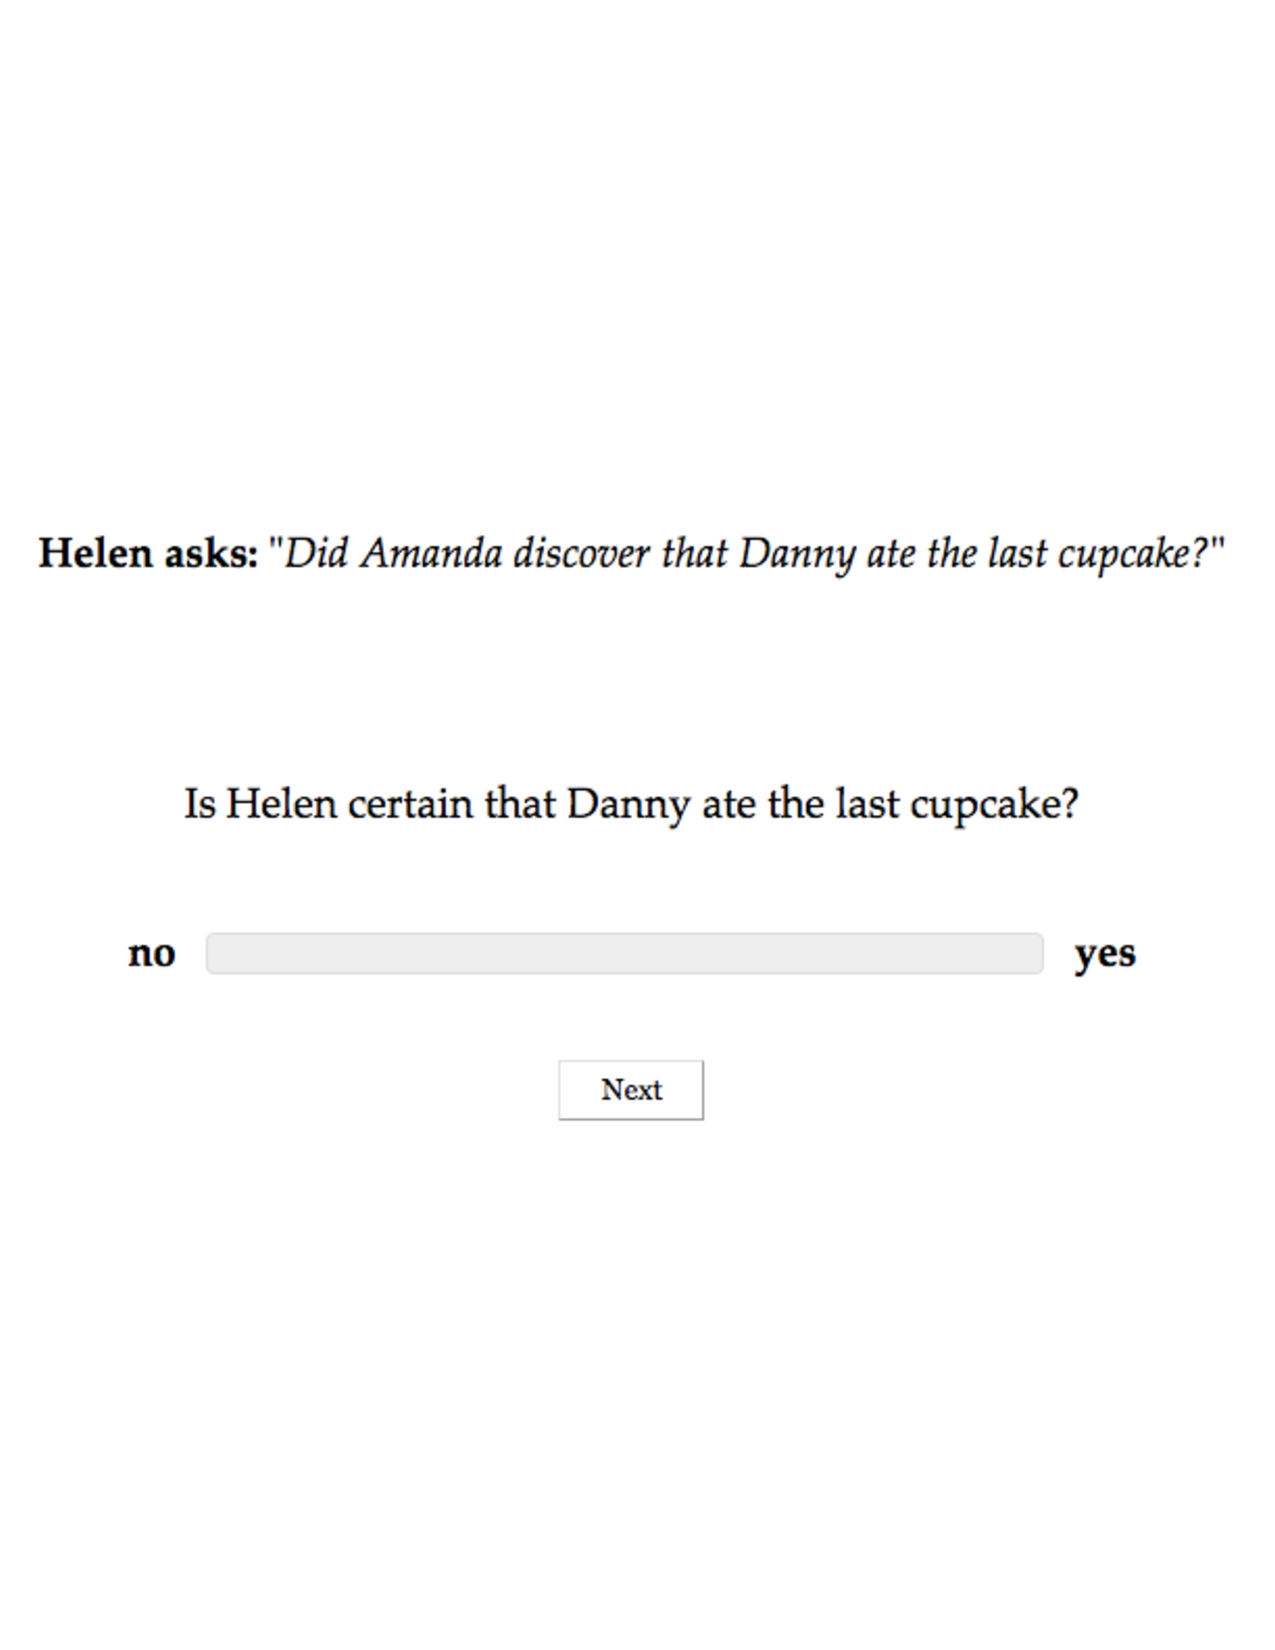
\includegraphics[width=10cm]{figures/trial-exp1}}
\end{center}
\caption{A sample trial in Experiment 1a}\label{fig-trial-exp1}
\end{figure}

After completing the experiment, participants filled out a short, optional survey about their age, their gender, their native language(s) and, if English is their native language, whether they are a speaker of American English (as opposed to, e.g., Australian or Indian English). To encourage them to respond truthfully, participants were told that they would be paid no matter what answers they gave in the survey.

\paragraph{Data exclusion}
Prior to analysis, the data from 13 participants who did not self-identify as native speakers of American English were excluded. To assess whether the remaining 287 participants attended to the task, we inspected their responses to the 6 control stimuli, for which we expected low responses. We excluded the data from 16 participants whose response means on the controls were more than 2 standard deviations above the group mean. We furthermore identified 5 participants whose variance in overall response distribution was more than 2 standard deviations below the mean by-participant variance: these participants always selected roughly the same point on the response scale. We excluded the data from these 5 participants, too, leaving data from 266 participants (ages 20-71; median: 36; 118 female, 143 male, 2 other, 3 undeclared).

\subsubsection{Results and discussion}\label{s22}

Figure \ref{f-projectivity} shows the mean certainty ratings for the target stimuli by predicate as well as for the main clause stimuli (abbreviated `MC'), in increasing order from left to right. The mean certainty ratings are largely consistent with impressionistic judgments reported in the literature. First, the ratings for main clause content are lowest overall, as expected for non-projective content. Second, the ratings for factive predicates are among the highest overall, suggesting comparatively high projectivity of the CC. Third, the mean certainty ratings of many optionally factive predicates are lower than those of many factive predicates and higher than those of main clauses as well as of non-veridical non-factives. However, Figure \ref{f-projectivity} also shows that the CCs of the 5 predicates assumed to be factive are not categorically more projective than the CCs of the optionally factive predicates, contrary to what is expected under the first definition of factive predicates. Specifically, the CCs of the optionally factive predicates {\em acknowledge, hear} and {\em inform} are at least as projective as the CCs of {\em reveal} or {\em discover}. This finding suggests that projectivity alone does not categorically distinguish factive predicates from optionally factive and non-factive ones.

\begin{figure}[H]
\centering

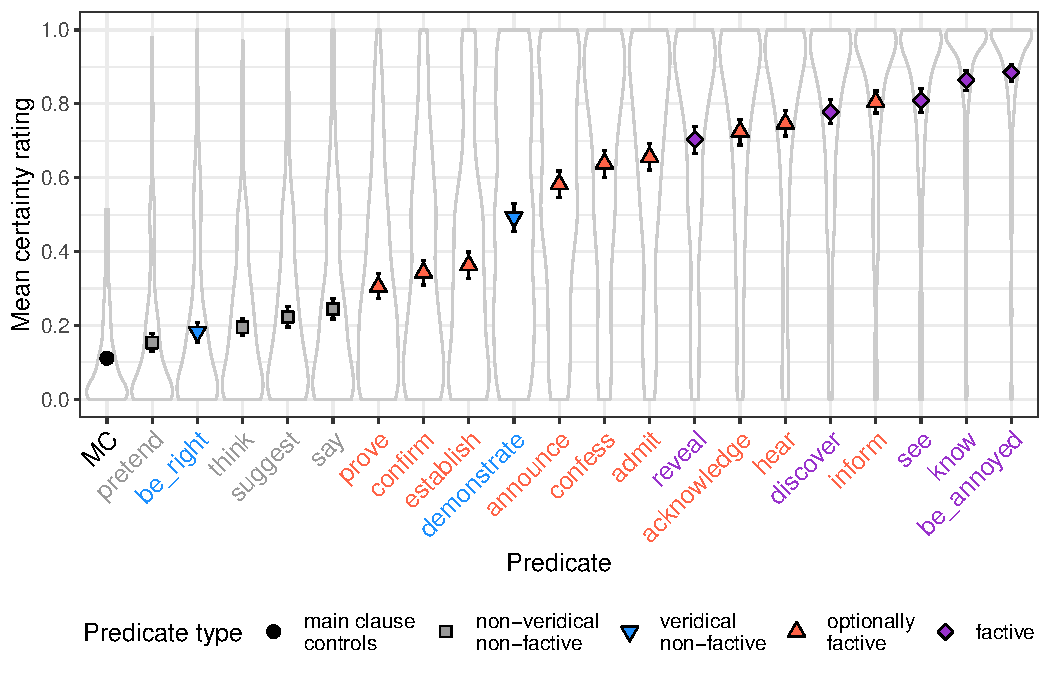
\includegraphics[width=.7\paperwidth]{../../results/5-projectivity-no-fact/graphs/means-projectivity-by-predicate-variability}

\caption{Mean certainty ratings by predicate in Exp.~1a. Error bars indicate 95\% bootstrapped confidence intervals. Light gray dots indicate individual participants' responses.} 
\label{f-projectivity}
\end{figure}




%1 acknowledge 0.725 0.0330  0.0339  0.692 0.758
% 2 admit       0.656 0.0390  0.0352  0.617 0.691
% 3 announce    0.582 0.0375  0.0370  0.545 0.619
% 4 be_annoyed  0.885 0.0220  0.0226  0.863 0.907
% 5 be_right    0.183 0.0271  0.0251  0.155 0.208
% 6 confess     0.639 0.0399  0.0376  0.599 0.676
% 7 confirm     0.343 0.0350  0.0358  0.308 0.379
% 8 MC          0.111 0.00895 0.00860 0.102 0.120
% 9 demonstrate 0.493 0.0403  0.0382  0.452 0.531
%10 discover    0.779 0.0303  0.0308  0.748 0.809
%11 establish   0.363 0.0340  0.0404  0.329 0.403
%12 hear        0.747 0.0371  0.0360  0.710 0.783
%13 inform      0.805 0.0287  0.0305  0.776 0.836
%14 know        0.864 0.0269  0.0241  0.837 0.888
%15 pretend     0.153 0.0232  0.0276  0.130 0.181
%16 prove       0.305 0.0314  0.0289  0.273 0.334
%17 reveal      0.704 0.0377  0.0349  0.666 0.739
%18 say         0.245 0.0283  0.0287  0.216 0.273
%19 see         0.809 0.0330  0.0303  0.776 0.840
%20 suggest     0.223 0.0256  0.0253  0.197 0.248
%21 think       0.195 0.0236  0.0243  0.172 0.220


In view of this finding, one might ask whether the categorization of clause-embedding predicates assumed in (\ref{pred}) is correct: perhaps there is a different place in which a line can be drawn between factive and optionally factive predicates based on the projectivity of the CCs? The mean certainty ratings plotted in Figure \ref{f-projectivity} suggest that this cannot be done in a non-arbitrary way. For instance, one might consider all predicates factive whose CC is at least as projective as that of {\em reveal}: this would mean that the predicates typically taken to be factive are factive, as well as {\em acknowledge, hear} and {\em inform}. There is, however, no principled reason why the projectivity of the CC of {\em reveal} should be the cut-off for factivity. A different approach would be to pick an arbitrary mean certainty rating, say .8, and to categorize predicates whose CC has a mean certainty rating of at least .8 as factive and predicates whose CC has a mean certainty rating below .8 as optionally factive. However, this is as unprincipled an approach as the previous one -- one could just as well pick a threshold of .85 or .75, with the result that different predicates would be considered factive: for instance, {\em discover} (mean: .78) would not count as factive with a threshold of .8, but would with a threshold of .75, and {\em see} (mean: .81) would count as factive with a threshold of .8, but not with a threshold of .85.\footnote{Choosing an arbitrary numeric threshold for factivity is also complicated by the fact that there is by-experiment variation in mean certainty ratings. For instance, the mean certainty ratings in Exp.~1a were lower, overall, than the mean certainty ratings in \citetpos{tbd-variability} Exps.~1. For example, the CC of {\em be annoyed}, which was the most projective in both sets of experiments, received mean certainty ratings of .96  and .92 in \citetpos{tbd-variability} Exps.~1a and 1b, respectively, but only a .86 in our Exp.~1a. This difference may be due to the fact that \citet{tbd-variability} primarily investigated highly projective content whereas our Exp.~1a included a wide range of less projective content: it is possible that participants' certainty ratings were influenced by the overall projectivity of the contents investigated. We leave this matter to future research.}

The possibility of categorizing clause-embedding predicates by the projectivity of the CC is further called into question by the fact that the CC of all of the 20 predicates investigated is projective, albeit to varying degrees, compared to the non-projective main clause controls. This was established by fitting a Bayesian mixed effects Beta regression model  with weakly informative priors using the \verb|brms| \citep{buerkner2017}  package in R \citep{R}.
The model predicted the certainty ratings from a fixed effect of predicate (with treatment coding and `main clause' as  reference level) and included the maximal random effects structure justified by the design: random by-participant and by-item intercepts (capturing random variability in projectivity between participants and between items, where an item is a unique combination of a predicate and a complement clause). \jt{A Beta regression model estimates two parameters of the outcome distribution: the mean  (like a linear regression model) as well as the precision. The precision is a measure of dispersion: the greater the precision, the more concentrated the ratings are around the mean. From the model we fitted, we obtain for each predicate a 95\% credible interval for the mean rating for that predicate: this allows us to identify whether the mean ratings of the predicate and of the main clause controls differ. We also obtain a 95\% credible interval for the precision coefficient: this allows us to identify whether the dispersion of ratings around the mean for the predicate and for the main clause controls differ.} Appendix \ref{modeldetails} motivates the use of Beta regression over linear regression, provides a brief primer on how to interpret Bayesian mixed effects Beta regression models and reports the full model output.

\jt{According to the Beta regression model, the estimated mean for each predicate was higher than that of the main clause controls, i.e., the 95\% credible intervals for the estimated mean did not contain 0 for any predicate. This finding suggests that the content of the complement of each of the 20 predicates is projective compared to non-projective main clause content. This finding is strengthened by the estimated precision coefficients:} with the exception of the predicates \emph{pretend},  \emph{think}, \emph{suggest} and \emph{say}, the estimated precision coefficient for each predicate was lower than that of the main clause controls (i.e., the 95\% credible intervals for the precision coefficient did not contain 0 for any predicate). This means that there was greater dispersion in certainty ratings these predicate than for the main clause controls; 

for the main clause controls than for all predicates except the above mentioned; that is, there is overall less uncertainty about the precise rating for these predicates than for the main clause controls.

 \jt{what? does precision really provide greater confidence in the claim that is supported by the mean or should we only report the mean findings}.\footnote{A Bayesian mixed effects linear regression with the same fixed and random effects structure yielded qualitatively identical results, except that the contrast between \emph{pretend} and the main clause controls was only marginally significant.}  

In sum, the findings of Exp.~1a suggest that the CC of the 20 clause-embedding predicates are projective: speakers who utter an interrogative with one of the 20 clause-embedding predicates are more committed to the CC than to main clause content.\footnote{According to \citet[1739]{spector-egre2015}, it is not clear whether the CC of {\em say} is projective. Our Exp.~1a findings suggest that it is weakly projective.}    Thus, to distinguish factive predicates from optionally factive and non-factive ones in this set of 20 predicates, one would need to distinguish one group of projective CCs from another group of projective CCs. The results suggest that there is no principled way of doing so.

It is possible that asking participants to assess projection with a gradient response scale encouraged them to provide non-categorical answers and that the observed projection variability is an artifact of the task. If so, categorically distinguishing factive predicates from others may be possible if participants were asked to assess projection with a categorical response task. To assess this possibility, we conducted Exp.~1b, which was identical to Exp.~1a but employed a two-alternative forced choice task.

\subsection{Experiment 1b: Categorical projection ratings}

\subsubsection{Methods}

\paragraph{Participants} 600 participants with U.S.\ IP addresses and at least 99\% of previous HITs approved were recruited on Amazon's Mechanical Turk platform. They were paid \$1.00 for participating.\footnote{Exps.~1a, 2a and 3a (gradient response task) were run in 2017 and 2018, whereas  Exps.~1b, 3a and 3b (categorical response task) were run in 2019. Participants in the later experiments were paid more to reflect an increased minimum wage in California.}


\paragraph{Materials and procedure} The materials and procedure were identical to those of Exp.~1a, with the exception of the task: participants responded `yes' or `no' to the question of whether the speaker is certain of the relevant content, as shown in Figure \ref{fig-trial-exp1b}.

\begin{figure}[h!]
\begin{center}
\fbox{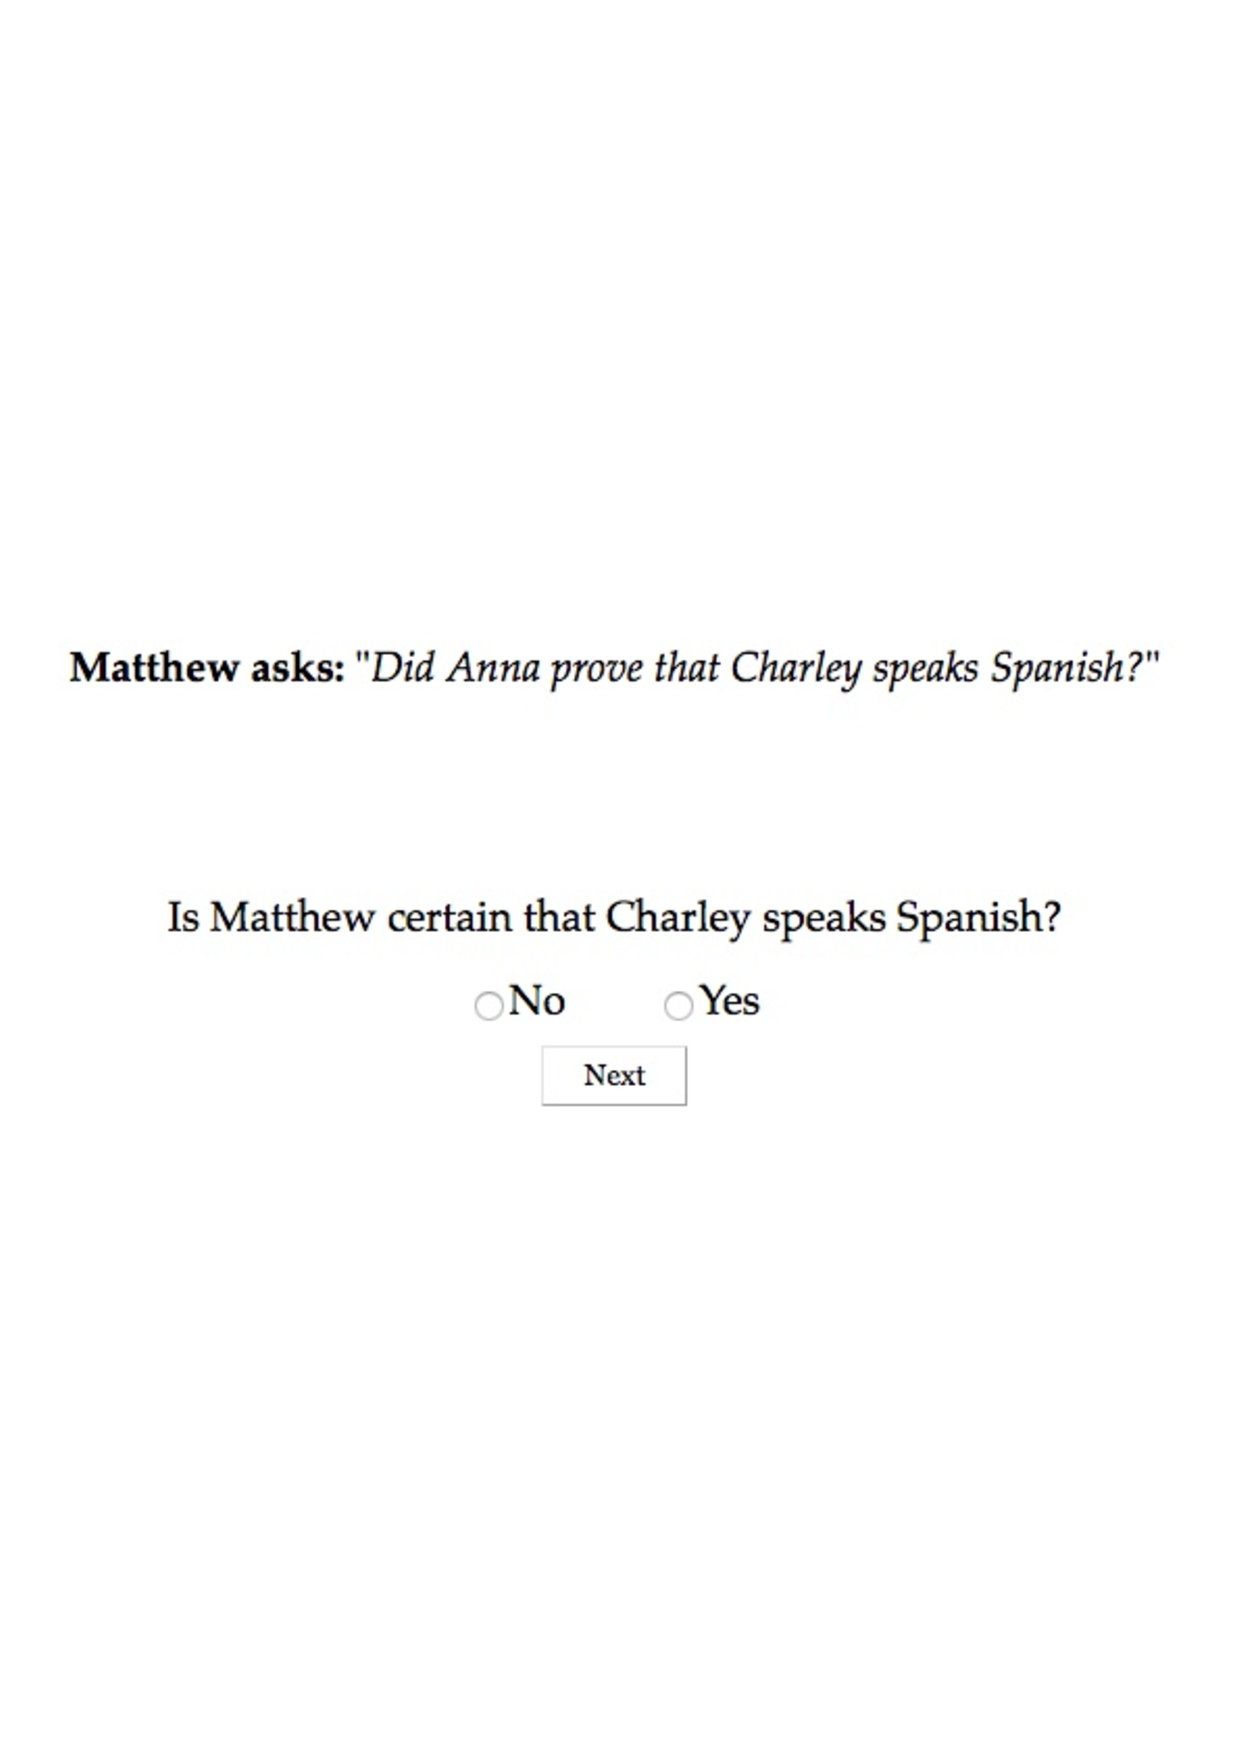
\includegraphics[width=10cm]{figures/Exp1b-trial}}
\end{center}
\caption{A sample trial in Experiment 1b}\label{fig-trial-exp1b}
\end{figure}

\paragraph{Data exclusion} For participants who took the experiment more than once, we only analyzed the data from the first time they took the experiment, leaving data from 525 participants. Prior to analysis, we excluded the data from 43 participants who did not self-identify as native speakers of American English. We also excluded the data from 46 participants who gave a wrong rating (`yes') to more than one of the six controls. The data from 436 participants (ages 18-81; median: 37; 207 female, 223 male, 2 other) entered the analysis. 

\subsubsection{Results and discussion}

Figure \ref{f-projectivity2} shows the proportion of `yes' ratings (indicating projection) for the predicates and the main clause stimuli, in increasing order from left to right. Jittered gray dots indicate the 436 individual participants' ratings. The order of predicates according to the projectivity of their CC in Exp.~1b is strikingly similar to that of Exp.~1a, as evidenced by the very high Spearman rank correlation of .983 (see Appendix \ref{a-comparison} for a visualization).\footnote{The Spearman rank correlation coefficient, a value between -1 and 1, is a nonparametric measure of rank correlation: the higher the coefficient, the more the relation between the the two variables can be described using a monotonic function; if the coefficient is positive, the value of one variable tends to increase with an increase in the other. In the case of our experiments, a coefficient of 1 would mean that there is a perfectly monotone increasing relation between the ranking of the predicates in Exp.~1a and Exp.~1b: for any two predicates $p_1$ and $p_2$, if $p_1$ ranks below $p_2$ in Exp.~1a (that is, the mean certainty rating of $p_1$ is lower than that of $p_2$), then that ranking is preserved in Exp.~1b.} 

The critical findings of Exp.~1a were replicated. First, the CCs of the factive predicates were not categorically more projective than the CCs of the optionally factive predicates:  the CCs of {\em acknowledge, hear} and {\em inform} were again at least as projective as the CCs of {\em reveal} or {\em discover}. Second, a non-arbitrary line between factive and optionally factive predicates cannot be drawn: the CCs of all 20 predicates were projective compared to the non-projective main clause controls. This was established by fitting a Bayesian mixed effects logistic regression model  with weakly informative priors using the \verb|brms| package in R. The model predicted the log odds of a `yes' over a `no' response from a fixed effect of predicate (with treatment coding and `main clause' as  reference level) and included the maximal random effects structure justified by the design, random by-participant and by-item intercepts. The estimated log odds of a `yes' response was greater for each predicate than that of the main clause controls, i.e., the 95\% credible intervals for the estimated coefficients did not contain 0 for any predicate. See Appendix \ref{a-comparison} \jd{insert correct ref} for model details. Thus, like Exp.~1a, the results of Exp.~1b do not support the assumption of the definition of factive predicates in (\ref{def}a) that factive predicates are categorically distinguished from optionally factive and non-factive ones by the projectivity of the CC.

\begin{figure}[H]

\centering
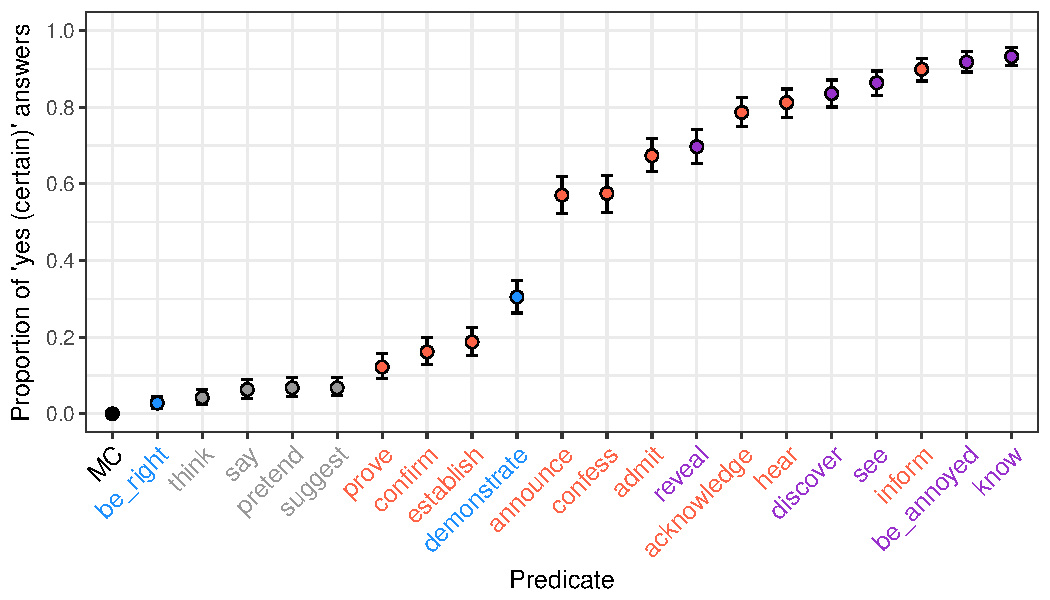
\includegraphics[width=.7\paperwidth]{../../results/8-projectivity-no-fact-binary/graphs/proportion-by-predicate-variability}
\caption{Proportion of `yes' ratings by predicate in Exp.~1b. Error bars indicate 95\% bootstrapped confidence intervals.}
\label{f-projectivity2}

\end{figure}


\subsection{Converging evidence for failure of projection-based definition of factive predicates}\label{s-converging1}

The findings of our Exps.~1a and 1b suggest that the definition of factive predicates in (\ref{def}a), according to which a predicate is factive if and only if its CC is presupposed, fails to identify a class of factive predicates. Converging evidence comes from three additional datasets: the CommitmentBank (\citealt*{demarneffe-etal-sub23}), the MegaVeridicality dataset (\citealt{white-rawlins-nels2018,white-etal2018b}) and the VerbVeridicality dataset (\citealt{ross-pavlick2019}).\footnote{We re-plotted the data, obtained at \url{https://github.com/mcdm/CommitmentBank}, \url{http://megaattitude.io} and \url{https://github.com/alexisjihyeross/verb_veridicality}, respectively. For the analysis files, see the aforementioned GitHub repository.}

The CommitmentBank is a collection of 1,200 naturally occurring English discourses from the Wall Street Journal, the British National Corpus and the Switchboard corpus: each discourse consists of a target sentence with a clause-embedding predicate embedded an entailment-canceling operator and up to two preceding context sentences, as illustrated in (\ref{cb}), with {\em know} in the target sentence embedded under negation:

\begin{exe}
\ex\label{cb} What fun to hear Artemis laugh. She's such a serious child. I didn't know she had a sense of humor. \\ \hspace*{.2cm} \hfill (\citealt[109]{demarneffe-etal-sub23})
\end{exe}
Annotators recruited on Amazon's Mechanical Turk platform provided certainty ratings for the CCs of the target sentences on a 7-point Likert scale labeled at three points: speaker/author is certain that the CC is true (coded as 3), speaker/author is not certain whether the CC is true or false (coded as 0), and speaker/author is certain that the CC is false (coded as -3); the lower half of the scale was included to differentiate speaker/author non-commitment to the CC from speaker/author commitment to the falsity of the CC (as may arise in, for instance, {\em I don't know that I agree.}). \citet{demarneffe-etal-sub23} assumed, for certainty ratings above 0, that the higher the certainty rating, the more projective the CC. Figure \ref{f-commitmentbank} shows the mean certainty ratings for the CCs in the 982 discourses with 45 non-veridical non-factive, optionally factive and factive clause-embedding predicates (target sentences embedded under non-epistemic modals were excluded; see \citealt[\S3]{demarneffe-etal-sub23}). In line with the findings of our Exps.~1, projection of the CC does not categorically distinguish factive predicates from optionally factive and non-factive ones: for instance, the CCs of the optionally factive predicates {\em foresee, confess, show, tell} and {\em accept} are at least as projective as those of some factive predicates. 

\begin{figure}[H]
\centering
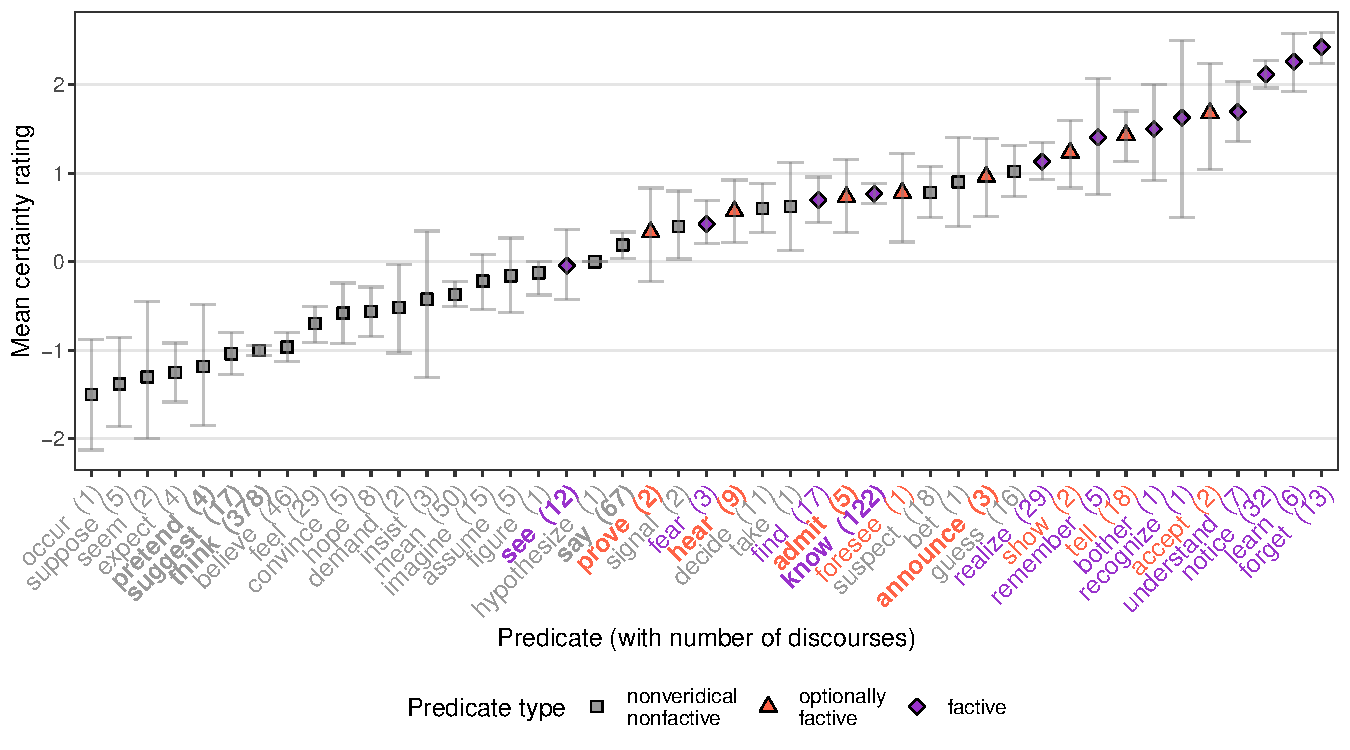
\includegraphics[width=.75\paperwidth]{../../CommitmentBank-analysis/graphs/means-projectivity-by-predicate-variability}

\caption{Mean certainty ratings by predicate, with number of discourses in parentheses, for 982 discourses in the CommitmentBank (\citealt*{demarneffe-etal-sub23}). Error bars indicate 95\% bootstrapped confidence intervals. Predicates included in our Exps.~1 given in bold.}
\label{f-commitmentbank}
\end{figure}

A second piece of evidence that the definition of factive predicates in (\ref{def}a) fails to identify a class of factive predicates comes from the VerbVeridicality dataset. This dataset includes 859 naturally occurring indicative matrix sentences with a total of 78 clause-embedding predicates and their clausal complements from the MultiNLI (\citealt{williams-etal2018}) corpus. To diagnose projection of the CC, negated variants of the 859 matrix sentences were created; an example is given in (\ref{vv-stim-proj}). For each negated variant, three participants rated on a 5-point Likert scale whether the CC is true given the target sentence; one endpoint of the scale was labeled `definitely true' (coded as 2) and the other `definitely not true' (coded as -2).\footnote{\citealt{ross-pavlick2019} investigated the extent to which the CCs follow from the indicative matrix sentences and from their negated counterparts. While they refer to both as `veridicality' inferences, the latter is typically called `projection' in the semantics/pragmatics literature.}

\begin{exe}
\ex\label{vv-stim-proj} The GAO has not indicated that it is unwilling to compromise.
\end{exe}

Figure \ref{f-vv-projectivity} plots the mean projectivity ratings for the CCs of the 78 predicates in the VerbVeridicality dataset, with labels for the 15 predicates from our experiments that are included in the MegaVeridicality dataset ({\em see} and {\em saw}, which are both included in the VerbVeridicality dataset, are plotted separately). As shown, projection of the CC does not categorically distinguish factive predicates from optionally factive and non-factive ones: the CCs of all of our optionally factive predicates are at least as projective as that of some factive predicate. 

\begin{figure}[H]
\centering
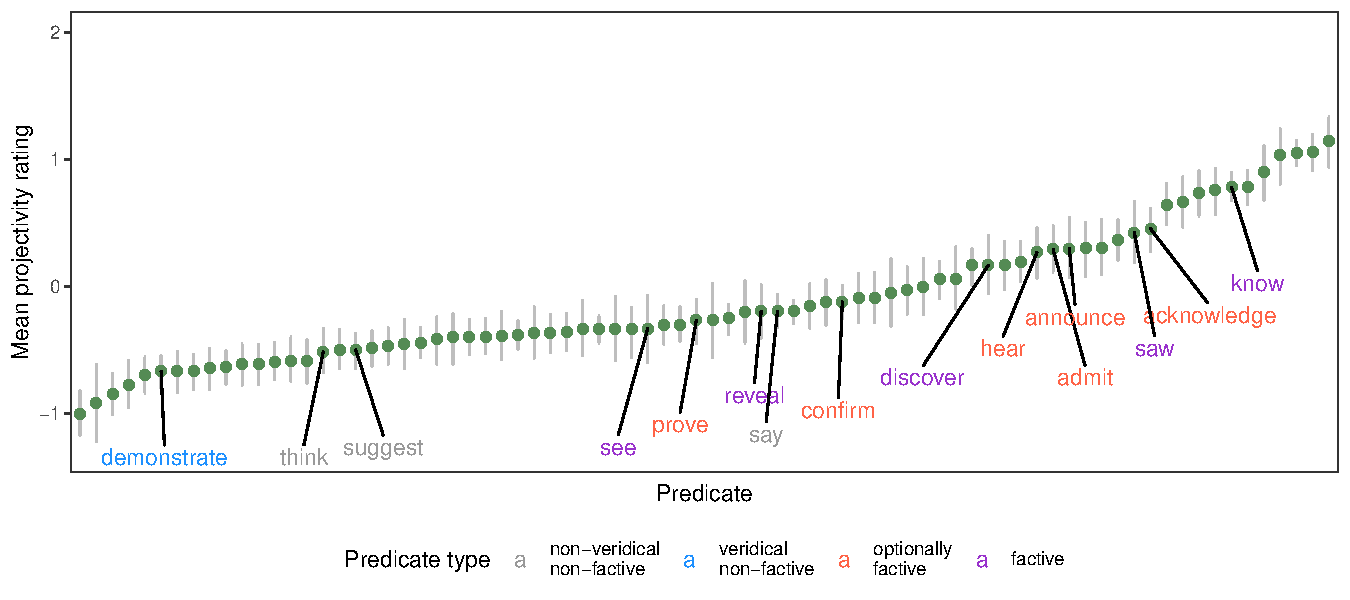
\includegraphics[width=.77\paperwidth]{../../VerbVeridicality-analysis/graphs/means-projection-by-predicate}

\caption{Mean projectivity rating by predicate in green, with 95\% bootstrapped confidence intervals, for the 78 predicates in the VerbVeridicality dataset (\citealt{ross-pavlick2019}), with labels for the 15 predicates featured in our experiments.}
\label{f-vv-projectivity}
\end{figure}



A third piece of converging evidence comes from the MegaVeridicality dataset, which contains projection ratings for the CCs of 517 English clause-embedding predicates. The stimuli that participants rated consisted of combinations of these predicates with low content arguments, as shown in (\ref{wr-stim-proj}) for {\em know}: the predicates and their clausal complements were embedded under negation in stimuli like (\ref{wr-stim-proj}a) and under negation, in the antecedent of a conditional and under the question operator in stimuli like (\ref{wr-stim-proj}b). To assess projection, participants were asked to respond to the question {\em Did that thing happen?} for stimuli like (\ref{wr-stim-proj}a) and to respond to the question posed by stimuli like (\ref{wr-stim-proj}b). The response options were `yes', `maybe or maybe not' and `no'. 

\begin{exe}
\ex\label{wr-stim-proj}
\begin{xlist}
\ex Somebody didn't know that a particular thing happened.
\ex If somebody didn't know that a particular thing happened, did that thing happen?
\end{xlist}
\end{exe}

The CCs of each of the 517 predicates in the MegaVeridicality dataset received between 29 and 60 projectivity ratings (mean: 32). To plot the ratings, we coded a `yes' response as 1 (the speaker is certain that the thing happened),  a `maybe or maybe not' response as 0 (the speaker is not certain whether the thing happened) and a `no' response as -1 (the speaker is certain that the thing didn't happen). Figure \ref{f-white-rawlins-projectivity} plots the mean projectivity ratings for the 517 predicates in the MegaVeridicality dataset, with labels for the 19 predicates from our experiments that are included in the MegaVeridicality dataset ({\em be right} is not included). As shown, projection of the CC does not categorically distinguish factive predicates from optionally factive and non-factive ones: for instance, the CCs of the optionally factive predicates {\em confess, acknowledge, admit, announce, hear} and {\em inform} are at least as projective as those of some factive predicates. 

\begin{figure}[H]
\centering
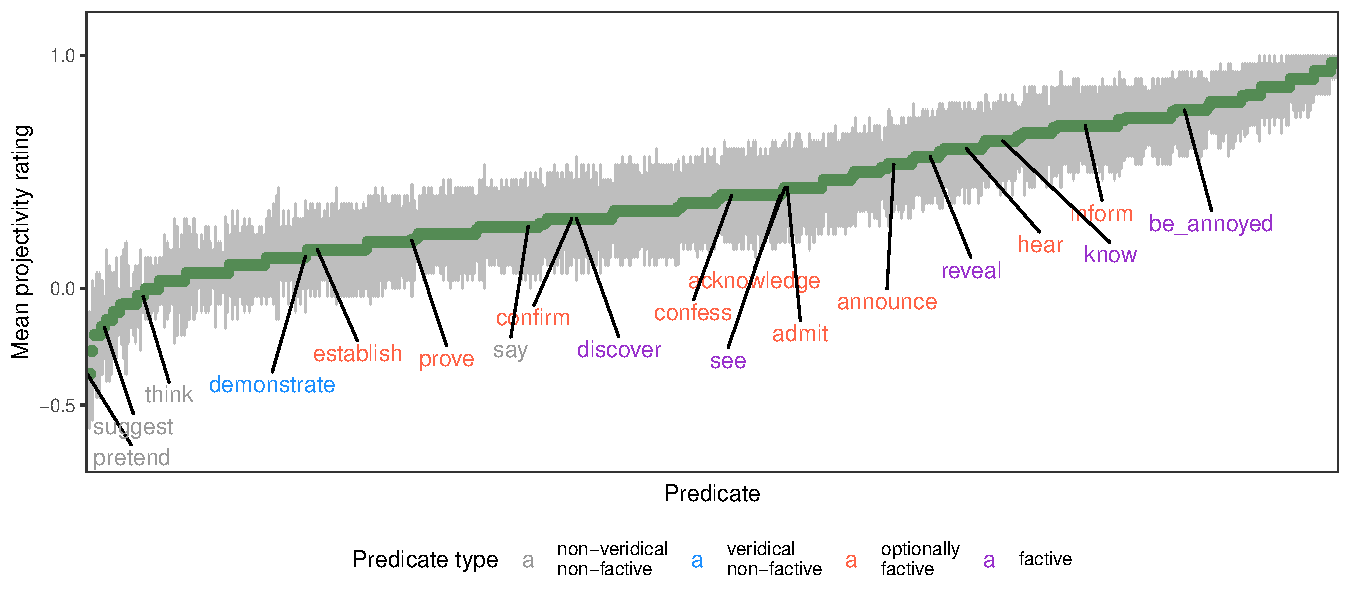
\includegraphics[width=.77\paperwidth]{../../MegaVeridicality-analysis/graphs/means-projection-by-predicate}

\caption{Mean projectivity rating by predicate in green, with 95\% bootstrapped confidence intervals, for the 517 predicates in the MegaVeridicality dataset (\citealt{white-rawlins-nels2018,white-etal2018b}), with labels for the 19 predicates featured in our experiments.}
\label{f-white-rawlins-projectivity}
\end{figure}


In sum, contrary to what is expected under the definition of factive predicates in (\ref{def}a), the findings of our Exps.~1a and 1b as well as those of the CommitmentBank, the VerbVeridicality and the MegaVeridicality datasets suggest that projection of the CC does not categorically distinguish factive predicates from optionally factive and non-factive ones. The challenge to the definition in (\ref{def}a) is compounded by the diversity of the empirical evidence: the evidence comes from constructed and naturally occurring examples, from examples presented to participants/annotators without a context to ones presented in context, from examples with diverse and minimal lexical content, from clause-embedding predicates embedded under a variety of entailment-canceling operators, and from projection ratings collected through different response tasks. We therefore conclude that the definition of factive predicates in (\ref{def}a), according to which a predicate is factive if and only if the content of the complement is presupposed, fails to identify a class of factive predicates. 

The experiments described in the next section were designed to explore whether the definition of factive predicates in (\ref{def}b), according to which entailment and projectivity jointly categorize clause-embedding predicates, is empirically supported. To this end, we collected entailment judgments for CCs of the same 20 predicates studied in Exps.~1.

\section{Experiments 2 and 3: Entailment}\label{s3}

Experiments 2 and 3 explored which of the CCs of the 20 clause-embedding predicates are entailed, to identify which predicates are factive under the definition of factive predicates in (\ref{def}b). We assume the standard definition of entailment, according to which entailment is a binary, categorical relation between two contents: given sentences $\phi$ and $\psi$, the content of $\phi$ entails the content of $\psi$ if and only if every world in which the content of $\phi$ is true is also a world in which the content of $\psi$ is true. If there is one world in which $\phi$ is true but $\phi$ is false, then the content of $\phi$ does not entail the content of $\psi$. 

To establish whether the content of an indicative matrix sentence with a clause-embedding predicate entails the CC, we used two standard diagnostics for entailment, given in (\ref{diag}). According to the `inference diagnostic' in (\ref{diag}a), the content of an indicative matrix sentence with a clause-embedding predicate entails the CC if and only if the CC definitely follows from a true statement of the matrix sentence. According to the `contradictoriness diagnostic' in (\ref{diag}b), an entailment relationship holds if and only an utterance of the indicative matrix sentence that is followed by a denial of the CC is contradictory. 

\begin{exe}
\ex\label{diag} Two diagnostics for entailment \hfill (see, e.g., \citealt[\S3.1]{ccmg90})
\begin{xlist}
\ex  Inference diagnostic (Exps.~2a and 2b)\\ $\phi$ entails $\psi$ if and only if, if $\phi$ is true, then the truth of $\psi$ definitely follows. 

\ex  Contradictoriness diagnostic  (Exps.~3a and 3b)\\ $\phi$ entails $\psi$ if and only if sentences of the form {\em $\phi$ and not $\psi$} are contradictory. 

\end{xlist}
\end{exe}
These two diagnostics for entailment were applied to the CCs of the 20 clause-embedding predicates in Exps.~2a/2b and Exps.~3a/3b, respectively: the two versions of each experiment differed in whether participants provided a gradient response (a) or a categorical one (b).  Both sets of experiments included control stimuli for which the relevant contents stand in an entailment relation, that is, for which the relevant inference definitely follows (Exps.~2) and that are definitely contradictory (Exps.~3). We assume that the CC of a clause-embedding predicate is not entailed if responses to the CC are significantly different from responses to these control stimuli and that the CC of a clause-embedding predicate is entailed if responses to the CC are not significantly different from responses to these control stimuli. Thus, identifying entailed CCs  requires arguing from a null result: given the standard classification of the 20 clause-embedding predicates in (\ref{pred}), we expect the CCs of factive and veridical non-factive predicates to be entailed, i.e., not significantly different from the control stimuli.

%Given this definition, establishing that the contents of two natural language sentences $\phi$ and $\psi$ do not stand in an entailment relation involves identifying a world in which the content of $\phi$ is true and the content of $\psi$ is false. 

%\jd{the following sentence is rhetorically a little weird: aren't we precisely interested in identifying when there \emph{is} an entailment relationship? the way it's framed makes it sound liike we're mostly interested in showing non-entailment. -- more generally, do we need all the detail of this paragraph or can we just move directly to the next paragraph, which introduces the standard diagnostics for entailment?} In this paper, however, we are also interested in establishing that the contents of two sentences $\phi$ and $\psi$  do stand in an entailment relation. Establishing this is straightforward if the content of some expression in $\phi$ denotes a subset of the content of some expression in $\psi$: for instance, in (\ref{ent1}a),  the content of $\phi$ entails the content of $\psi$ because the denotation of {\em black cat} in $\phi$ is a subset of the denotation of {\em cat} in $\psi$. No such structural relation exists, however, between the content of a sentence with a clause-embedding predicate and the CC, as in (\ref{ent1}b). %Furthermore, it is of course impossible to empirically verify that the content of $\phi$ entails the content of $\psi$ in (\ref{ent1}b) because it is impossible to verify that $\psi$ is true in all worlds in which $\phi$ is true. 
%
%\begin{exe}
%\ex\label{ent1}
%\begin{xlist}
%\ex $\phi$: Sam owns a black cat. \hspace*{1.5cm} $\psi$: Sam owns a cat.
%
%\ex $\phi$: Sam knows that it's raining. \hspace*{.6cm} $\psi$: It's raining.
%
%\end{xlist}
%\end{exe}

%\footnote{\citealt{sudo-thesis} proposed to diagnose whether a presupposition is an entailment based on whether the presupposition obligatorily restrict the domain of the quantifier {\em exactly one}. According to this diagnostic, the pre-state content of {\em stop} is a presupposition and an entailment because (ia) means that exactly one student who used Mac stopped using Mac. On the other hand, the gender presupposition of {\em she} in (ib) is not an entailment because (ib) does not mean that exactly one female student criticized herself, but that exactly one student criticized herself (see \citealt{zehr-schwarz2016,zehr-schwarz2018} for some experimental support). According to this diagnostic, the CC of {\em know} is entailed content: (ic) means that exactly one student who got accepted by MIT knows that they got accepted by MIT. {\bf REVISE THIS: Whether the {\em exactly one} diagnostic can help settle the debate about which contents of complements of clause-embedding predicates are entailed is a question we leave for future research.}
%
%\begin{exe}
%\exi{(i)} 
%\begin{xlist}
%\ex Exactly one student stopped using Mac. \hfill (\citealt[59]{sudo-thesis})
%
%\ex Exactly one student criticized herself. \hfill (\citealt[61]{sudo-thesis})
%
%\ex Exactly one student knows that they got accepted by MIT. \hfill (\citealt[64]{sudo-thesis})
%
%\end{xlist}
%\end{exe}}

\subsection{Exp.~2a: Gradient ratings using the inference diagnostic for entailment}\label{s31}

Exp.~2a investigated which of the CCs of the 20 clause-embedding predicates are entailed based on the inference diagnostic for entailment in (\ref{diag}a). Participants assessed on a gradient scale whether the CC follows from true statements of indicative matrix sentences with the 20 clause-embedding predicates.

%In contrast to the entailment relationship, which is categorical and categorical, the inference relationship is gradient: given true statements $\phi_1$ and $\phi_2$, the inference to the truth of $\psi$ may be stronger from $\phi_1$ than from $\phi_2$. To illustrate assume that $\phi_1$ is the sentence {\em Julian is from Cuba} and that $\phi_2$ is the sentence {\em Julian is from Germany}: the inference to the truth of $\psi$ {\em Julian dances salsa} is stronger from $\phi_1$ than from $\phi_2$.

% To illustrate, assume that Chris wears his pajamas when he is at home and that he doesn't wear pajamas outside of his home. Now consider the sentences $\phi_1$ to $\phi_5$ in (\ref{chris}). Given the aforementioned assumption, the truth of the content of the statement $\psi$ {\em Chris is wearing his pajamas} definitely follows from a true statement of $\phi_1$\jd{is this true? -- the way the assumption is formulated above, it's a habitual -- ie, he habitually wears pajamas at home and not outside the home; but presumably, there is a point in time at which he changes from pajamas to outside clothes, so he doesn't wear just pajamas at home, so it doesn't follow from $\phi_5$ that Chris is wearing pajamas}, it follows to increasingly lower degrees from true statements of $\phi_2$ to $\phi_4$ and it does not follow from a true statement of $\phi_5$. 
%
%\begin{exe}
%\ex\label{chris}
%\begin{xlist}
%\exi{$\phi_1$} Chris is at home.
%\exi{$\phi_2$} Chris is likely at home.
%\exi{$\phi_3$} Chris is possibly at home.
%\exi{$\phi_4$} There is a slight possibility that Chris is at home.
%\exi{$\phi_5$} Chris is not at home.
%\end{xlist}
%\end{exe}

\subsubsection{Methods}

\paragraph{Participants} 300 participants with U.S.\ IP addresses and at least 99\% of previous HITs approved were recruited on Amazon's Mechanical Turk platform (ages: 19-69, median: 36; 152 female, 148 male). They were paid \$0.75 for participating.

\paragraph{Materials} The target stimuli were 400 indicative matrix sentences: they were constructed by combining the 20 clause-embedding predicates with the 20 complement clauses (for 400 predicate/clause combinations, as in Exps.~1) and a random proper name subject whose gender differed from the gender of the proper name subject of the embedded clause. As illustrated in the sample stimuli in (\ref{stims2}), these matrix sentences were presented to participants as true statements. For each of the 400 target stimuli, the inference that was tested was the inference to the CC: for instance, participants were asked about (\ref{stims2}a) whether it follows that Danny ate the last cupcake and about (\ref{stims2}b) whether it follows that Emma studied on Saturday morning.

\begin{exe}
\ex\label{stims2}
\begin{xlist}
\ex {\bf What is true:} Melissa knows that Danny ate the last cupcake.
\ex {\bf What is true:} Jerry pretended that Emma studied on Saturday morning.
\end{xlist}
\end{exe}

The experiment included eight control stimuli that were used to assess whether participants were attending to the task and interpreted the task correctly, as well as to identify inference ratings for entailed content. For the four entailing control stimuli in (\ref{control-good2}), the tested inferences are entailments of the true statements: in (\ref{control-good2}a), for instance, that Frederick solved the problem is an entailment of the true statement that Frederick managed to solve the problem. We expected the inference ratings for these four control stimuli to be at ceiling and, as discussed above, we rely on the ratings for these stimuli to identify entailments. In contrast, the inferences tested with the four non-entailing control stimuli in (\ref{control-bad2}) definitely do not follow from these true statements: for instance, in (\ref{control-bad2}a), that Dana wears a wig does not follow from Dana watching a movie last night. We expected the inference ratings for these four control stimuli to be at floor.

\begin{exe}
\ex\label{control-good2} Entailing control stimuli
\begin{xlist}
\ex {\bf What is true:} Frederick managed to solve the problem. (Tested inference: Frederick solved the problem.)
\ex {\bf What is true:} Zack bought himself a car this morning. (Tested inference: Zack owns a car.)
\ex {\bf What is true:} Tara broke the window with a bat. (Tested inference: The window broke.)
\ex {\bf What is true:} Vanessa happened to look into the mirror. (Tested inference: Vanessa looked into the mirror.)
\end{xlist}
\ex\label{control-bad2} Non-entailing control stimuli
\begin{xlist}
\ex {\bf What is true:} Dana watched a movie last night. (Tested inference: Dana wears a wig.)
\ex {\bf What is true:} Hendrick is renting an apartment. (Tested inference: The apartment has a balcony.)
\ex {\bf What is true:} Madison was unsuccessful in closing the window. (Tested inference:  Madison closed the window.)
\ex {\bf What is true:} Sebastian failed the exam. (Tested inference: Sebastian did really well on the exam.)
\end{xlist}
\end{exe}

Each participant saw a random set of 28 stimuli: each set contained one target stimulus for each of the 20 predicates (each with a unique complement clause) and the same 8 control stimuli. Trial order was randomized.

\paragraph{Procedure} Participants were told that they would read true statements and that they would be asked to assess whether a second statement follows from that true statement. On each trial, participants read the true statement and were asked to respond to the question {\em Does it follow that\ldots?}, with the complement clause realized by the complement clause of the clause-embedding predicate. Participants responded on a sliding scale from `definitely doesn't follow' (coded as 0) to `definitely follows' (coded as 1), as shown in Figure \ref{f-trial-exp3}.

\begin{figure}[H]
\begin{center}
\fbox{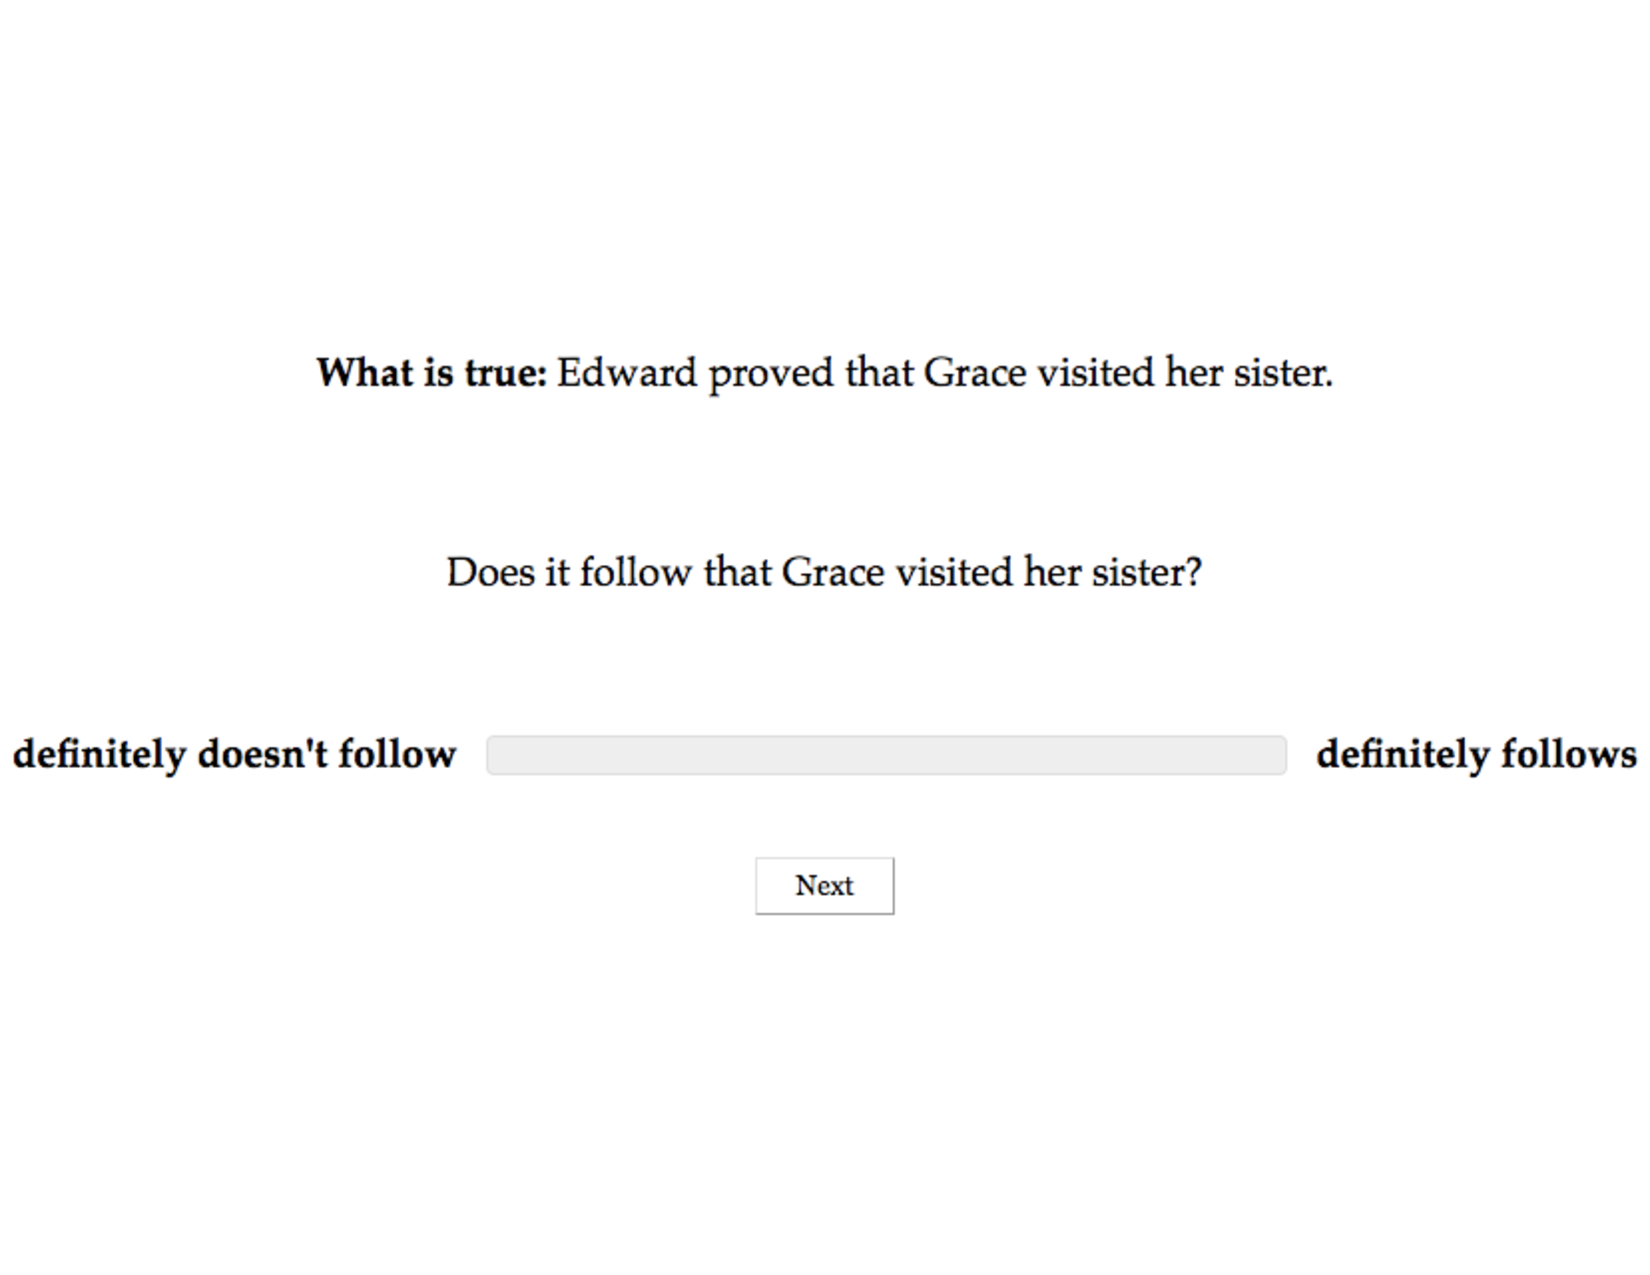
\includegraphics[width=13cm]{figures/inference-trial}}
\end{center}
\caption{A sample trial in Experiment 2a}\label{f-trial-exp3}
\end{figure}

To familiarize participants with the task, they first responded to the two familiarization stimuli in (\ref{train2}), where the inference tested was the CC. Participants who rated (\ref{train2}a) in the lower half of the sliding scale or (\ref{train2}b) in the upper half of the sliding scale were given an explanation for why their answer was wrong. Participants could only advance to the 28 stimuli if they gave a plausible rating to the two familiarization stimuli, that is, a rating in the upper half of the scale for (\ref{train2}a) and in the lower half for (\ref{train2}b).

\begin{exe}
\ex\label{train2}
\begin{xlist}
\ex {\bf What is true:} Drew is correct that Patty lives in Canada. 

\ex {\bf What is true}: Drew believes that Patty lives in Canada.
\end{xlist}
\end{exe}

After responding to the 28 stimuli, participants filled out a short, optional survey about their age, their gender, their native language(s) and, if English is their native language, whether they are a speaker of American English (as opposed to, e.g., Australian or Indian English). To encourage them to respond truthfully, participants were told that they would be paid no matter what answers they gave in the survey.

\paragraph{Data exclusion}

Prior to analysis, the data from 14 participants who did not self-identify as native speakers of American English were excluded. For the remaining 286 participants, we inspected their responses to the 8 control stimuli. The group mean for the four control stimuli in (\ref{control-good2}), for which the strength of the inference was expected to be at ceiling, was .94. The group mean for the four control stimuli in (\ref{control-bad2}), for which the strength of the inference was expected to be at floor, was .05. These group means suggest that, overall, participants attended to and understood the task. The response means of 27 participants were more than 2 standard deviations below the group mean for the control stimuli in (\ref{control-good2}) or above the group mean for the control stimuli in (\ref{control-bad2}). Closer inspection revealed that these participants' responses to the control stimuli were systematically higher or lower, respectively, suggesting that these participants did not attend to the task or interpreted the task differently. The data from these 27 participants were also excluded. In this experiment, we did not identify any participants who always selected roughly the same point on the response scale. The results presented below are based on data from 259 participants (ages 19-69; median: 36; 132 female, 128 male). %; the group means were .96 for the control stimuli in (\ref{control-good2}) and .03 for the control stimuli in (\ref{control-bad2}).

\subsubsection{Results}


Figure \ref{f-veridicality-predicate} plots the mean inference ratings for the target stimuli by predicate, in increasing order from left to right, as well as for the non-entailing and entailing controls. In line with impressionistic judgments reported in the literature, the mean inference ratings for most factive predicates as well as the veridical non-factive predicate {\em be right} are quite high, suggesting strong inferences to the truth of the CC. The mean inference ratings of the purportedly factive predicate {\em reveal} and of the purportedly veridical non-factive predicate {\em demonstrate} are lower, suggesting comparatively weaker inferences to the truth of the CC. 

\begin{figure}[h!]
\centering

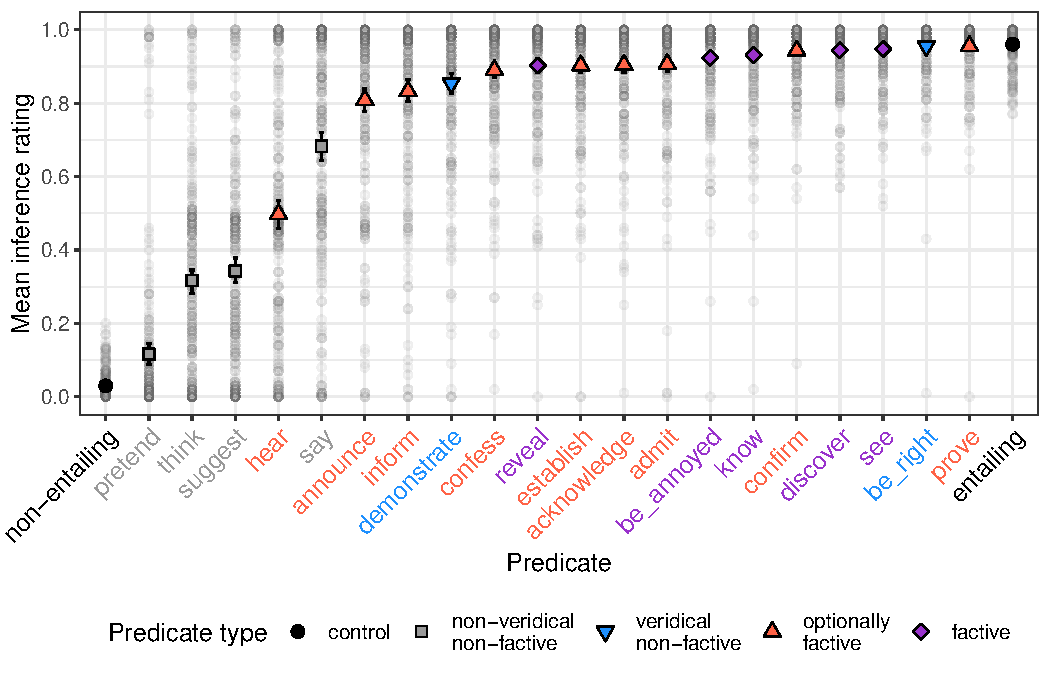
\includegraphics[width=.7\paperwidth]{../../results/4-veridicality3/graphs/means-inference-by-predicate-variability}

\caption{Mean inference rating by predicate in Exp.~2a, including the non-entailing and entailing controls. Error bars indicate bootstrapped 95\% confidence intervals. Light gray dots indicate individual participants' ratings.} 
\label{f-veridicality-predicate}
\end{figure}

\jt{The qualitative observations were borne out by a Bayesian mixed effects Beta regression model with weakly informative priors using the} \verb|brms| \jt{package in R. The model predicted the inference ratings from a fixed effect of predicate (with treatment coding and `entailing control' as  reference level) and included the maximal random effects structure justified by the design: random by-participant and by-clause intercepts (capturing random variability in inference ratings between participants and between complement clauses) and random by-participant and by-clause slopes for the fixed effect of predicate (capturing that the effect of predicate on inference ratings may vary across participants and complement clauses).} See appendix \ref{modeldetails} for the full model output.

\jt{According to the Beta regression model, the estimated mean of all predicates except {\em } and {\em } was lower than that of the main clause controls (i.e., the 95\% credible intervals for the estimated mean did not contain 0 for any predicate). This finding suggests that the content of the complement of each of the 20 predicates is projective compared to non-projective main clause content. This finding is strengthened by the estimated precision coefficients:} with the exception of the predicates \emph{pretend},  \emph{think}, \emph{suggest} and \emph{say}, the estimated precision coefficient for each predicate was lower than that of the main clause controls (i.e., the 95\% credible intervals for the precision coefficient did not contain 0 for any predicate). This means that there was greater dispersion in certainty ratings for the main clause controls than for all predicates except the above mentioned; that is, \jt{what? does precision really provide greater confidence in the claim that is supported by the mean or should we only report the mean findings}.\footnote{A mixed effects linear regression \jt{with the same fixed and random effects structure} yielded qualitatively identical results, except that the contrast between \emph{pretend} and the main clause controls was only marginally significant.} 

Of the 20 predicates, only the ratings for the CCs of {\em be right} and {\em prove} are not different from those of the entailing controls. For the CCs of {\em see, discover} and {\em confirm}, the ratings were slightly lower but the precision was not measurably different from that of the entailing controls, meaning that the ratings for the CCs of these predicates are extremely similar to those of the entailing controls but slightly lower on average. Thus, the gradient inference ratings for the CCs of {\em be right, prove, see, discover} and {\em confirm} are compatible with the assumption that the CCs of these predicates are entailed. The inference ratings for the remaining predicates, including the factive predicates {\em know, be annoyed} and {\em reveal} and the veridical non-factive predicate {\em demonstrate}, are significantly lower: this finding suggests that these CCs are not entailed, contrary to assumption. 



\subsubsection{Discussion}

The findings of Exp.~2a have two unexpected implications. The first one concerns the predicates for which Exp.~2a found that their CCs are entailed, namely {\em confirm, discover, see, be right} and {\em prove}. Given definition (\ref{def}b), according to which a predicate is factive if and only if its CC is presupposed and entailed, this means that these five predicates are factive, if their CCs are presupposed. As discussed above, Exps.~1 found that the CCs of all 20 predicates investigated is at least mildly projective, compared to main clause content: we are therefore led to the conclusion that, according to the definition in (\ref{def}b), all five of these predicates are factive! This is an unsatisfying conclusion because this set of predicates is not a natural class, given the tremendous differences in how projective the CCs of these predicates are: that of {\em be right} was the least projective, while that of {\em see} was highly projective. However, since a non-arbitrary cut-off point for projectivity cannot be identified (see the discussion in section \ref{s2}), there is no principled way of narrowing down this set, to result in a more homogenous class of factive predicates.

The second unexpected implication concerns some of the predicates for which Exp.~2a found that their CCs are not entailed, namely {\em know, be annoyed, reveal} and {\em demonstrate}. This finding means that, contrary to what is typically assumed, the predicates {\em know, be annoyed} and {\em reveal} are not factive under the definition of factive predicates in (\ref{def}b) and the predicate {\em demonstrate} is not veridical.

Our way of identifying entailed CCs, namely by comparing the CCs of the 20 predicates to entailed content, was motivated by the standard definition of entailment. One can, of course, ask whether there might be better ways of identifying entailed CCs. For instance, one might consider those CCs entailed whose mean inference rating was at least as high as that of {\em demonstrate} (.85): this would mean that the CCs of all of the predicates typically taken to be factive or veridical non-factive are entailed, as well as the CCs of some optionally factive predicates. There is, however, no principled reason why the ratings for the CC of {\em demonstrate} should be the threshold for entailment. One could also pick an arbitrary mean inference rating, say .9, and categorize CCs with mean ratings of at least .9 as entailed, and CCs with mean ratings below .9 as not entailed. Of course, this way of identifying entailed CCs is also not principled. After all, one could just as well pick a threshold of .95 or .85, with the result that the CCs of different predicates would be considered entailed: for instance, the CC of {\em reveal} (.9) would count as entailed with a threshold of .85 but not with a threshold of .95. Furthermore, neither of these alternative ways of identifying entailed CCs are compatible with the standard definition of entailment because, under both, one would need to allow for CCs to count as entailed even though they received significantly lower ratings than entailed content.

%          verb       Mean       YMin       YMax
%1  acknowledge 0.90471042 0.88624807 0.92131660
%2        admit 0.90694981 0.88829633 0.92567761
%3     announce 0.80899614 0.77883687 0.83727606
%4   be_annoyed 0.92389961 0.90810618 0.93962162
%5     be_right 0.95509653 0.94319788 0.96548359
%6      confess 0.89019305 0.87007239 0.90965830
%7      confirm 0.94332046 0.93138031 0.95390347
%8  demonstrate 0.85378378 0.82782625 0.87772683
%9     discover 0.94447876 0.93331853 0.95467471
%10 entailing C 0.96077220 0.95600193 0.96480743
%11   establish 0.90289575 0.88297104 0.91989286
%12        hear 0.49776062 0.45794208 0.53757529
%13      inform 0.83262548 0.80188803 0.86197201
%14        know 0.93127413 0.91589768 0.94494402
%15  non-ent. C 0.02969112 0.02574131 0.03395849
%16     pretend 0.11617761 0.08848263 0.14606274
%17       prove 0.95583012 0.94443919 0.96583205
%18      reveal 0.90262548 0.88347104 0.92123745
%19         say 0.68277992 0.64300193 0.72162548
%20         see 0.94764479 0.93698745 0.95795753
%21     suggest 0.34254826 0.30826158 0.37788127
%22       think 0.31633205 0.28609846 0.34965347

One might ask whether the finding of Exp.~2a that the CCs of {\em know, be annoyed, reveal} and {\em demonstrate} are not entailed is an artifact of the response task. It is possible, for instance, that the gradient response scale on which participants responded in Exp.~2a contributed to lower inference ratings for the CCs of these predicates, resulting in them being classified as not entailed. To assess this possibility, we conducted Exp.~2b, which was identical to Exp.~2a but employed a two-alternative forced choice task.

\subsection{Exp.~2b: Categorical ratings using the inference diagnostic for entailment}

\subsubsection{Methods}

\paragraph{Participants} 600 participants with U.S.\ IP addresses and at least 99\% of previous HITs approved were recruited on Amazon's Mechanical Turk platform. They were paid \$1 for participating.

\paragraph{Materials and procedure} The materials and procedure were identical to those of Exp.~2a, with the exception of the task: participants responded `yes' or `no' to the question of whether the CC follows from the true statement, as shown in Figure \ref{fig-trial-exp2b}.

\begin{figure}[h!]
\begin{center}
\fbox{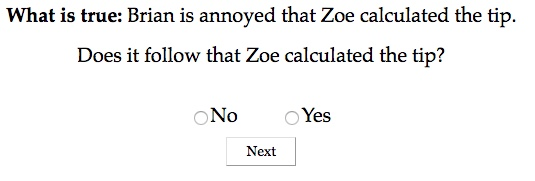
\includegraphics[width=10cm]{figures/Exp2b-trial}}
\end{center}
\caption{A sample trial in Experiment 2b}\label{fig-trial-exp2b}
\end{figure}


\paragraph{Data exclusion} For participants who took the experiment more than once, we only analyzed the data from the first time they took the experiment, leaving data from 431 participants. Prior to analysis, we excluded the data from 35 participants who did not self-identify as native speakers of American English. We also excluded the data from 25 participants who gave more than one wrong rating to one of the eight controls, where a wrong rating is a `yes' to a non-entailing control and a `no' to an entailing one. The data from 375 participants (ages 18-73; median: 38; 187 female, 187 male) entered the analysis below. 
    

\subsubsection{Results and discussion}

Figure \ref{fig:2bresults} shows the proportion of `yes' ratings by predicate, in increasing order from left to right, as well as on non-entailing and entailing controls. The findings of Exp.~2b are strikingly similar to those of Exp.~2a: the proportions of `yes' ratings are quite high for most factive predicates as well as the veridical non-factive predicate {\em be right}, but the proportions for the purportedly factive predicate {\em reveal} and the purportedly veridical non-factive predicate {\em demonstrate} are lower. The very high Spearman rank correlation of .989 between Exps.~2a and 2b shows that the order of the predicates is almost entirely identical between the gradient and the categorical inference measure (see Appendix \ref{a-comparison} for a visualization). 
 
\begin{figure}[H]
\centering
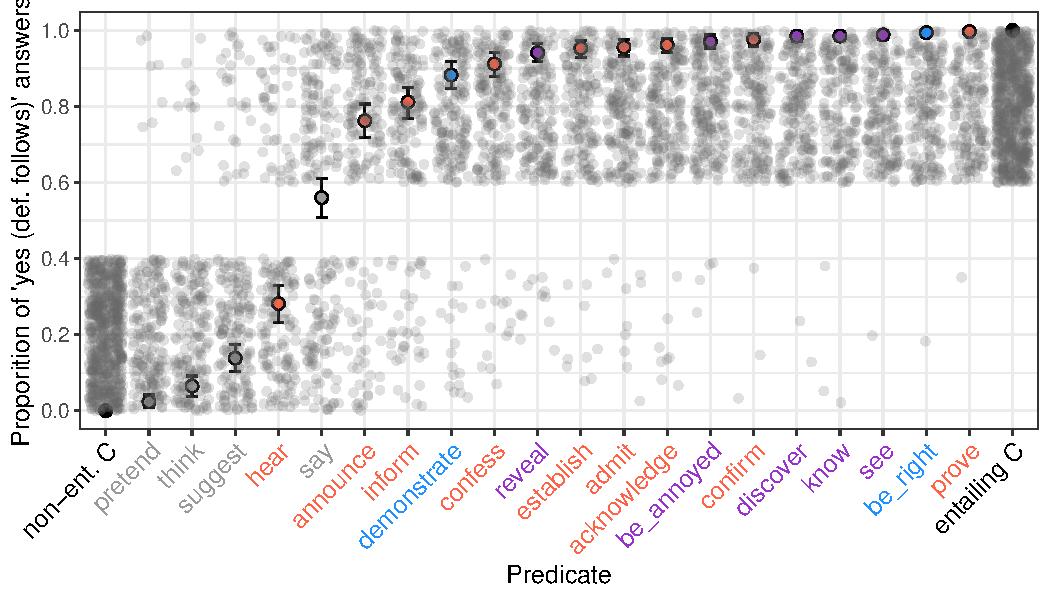
\includegraphics[width=.7\paperwidth]{../../results/7-veridicality3-binary/graphs/proportion-by-predicate-variability-individual}

\caption{Proportion of `yes' ratings by predicate in Exp.~2b. Error bars indicate 95\% bootstrapped confidence intervals. Jittered light gray dots indicate individual participants' ratings of `yes' (coded as 1) and `no' (coded as 0).}
\label{fig:2bresults}
\end{figure}

\jd{describe model and connect with text} In other words, the categorical inference ratings for the CCs of {\em prove, be right, know, see, discover} and {\em confirm} are indistinguishable from those of the entailing controls. This finding is compatible with the assumption that the CCs of these predicates are entailed. In contrast to Exp.~2a, the findings of Exp.~2b are compatible with the assumption that the CC of {\em know} is entailed. The categorical inference ratings for the CCs of the remaining predicates, including {\em be annoyed, reveal} and {\em demonstrate}, are significantly lower, suggesting that the CCs of these predicates are not entailed.

Changing the response task from a gradient one (Exp.~2a) to a categorical one (Exp.~2b) did not result in dramatically different findings:  the classification of the CC of only one of the 20 clause-embedding predicates changed, namely that of {\em know}. As a consequence, the findings of Exp.~2b have the same unexpected implications as those of Exp.~2a. First, according to the definition of factive predicates in (\ref{def}b), the set of predicates with entailed CCs, namely {\em confirm, discover, see, know, be right} and {\em prove}, are identified as factive. This set is not a natural class, given that the CC of {\em be right} was the least projective, while that of {\em know} was the most projective of the 20 predicates investigated. Second, the predicates {\em be annoyed} and {\em reveal} are not factive under the definition of factive predicates in (\ref{def}b) and the predicate {\em demonstrate} is not veridical. 


Because Exps.~2a and 2b differed in the response task, these findings cannot be attributed to the response task. One might ask whether these findings are an artifact of the inference diagnostic for entailment. To assess this possibility, we conducted Exps.~3a and 3b, which were identical to Exps.~2a and 2b, respectively, but employed the contradictoriness diagnostic for entailment.

\subsection{Exp.~3a: Gradient ratings using the contradictoriness diagnostic for entailment}\label{s32}

Exp.~3a investigated which of the CCs of the 20 clause-embedding predicates are entailed based on the contradictoriness diagnostic for entailment in (\ref{diag}b). Participants rated the contradictoriness of utterances of English sentences of the form {\em $\phi$ but not $\psi$}, where $\phi$ is an indicative matrix sentence with a clause-embedding predicate and $\psi$ is its clausal complement, as in (\ref{announce3}):

\begin{exe}
\ex\label{announce3} Mary announced that she is pregnant, but she's not.
\end{exe}
Gradient contradictoriness ratings were collected.

\subsubsection{Methods}

\paragraph{Participants} 300 participants with U.S.\ IP addresses and at least 99\% of previous HITs approved were recruited on Amazon's Mechanical Turk platform (ages: 18-72, median: 35; 137 female, 162 male, 1 other). They were paid \$0.75 for participating.

\paragraph{Materials} On target trials, the 400 predicate/clause combinations were combined with a random proper name subject and a {\em but-}clause that denied the truth of the CC. As shown in ({\ref{stims}), stimuli were presented to participants as utterances by named speakers. The proper names that realized the speakers, the subjects of the 20 predicates and the subjects of the complement clauses were all unique. The gender of the proper name subject of the predicate was distinct from the gender of the proper name in the complement clause, to ensure that the pronoun in the elliptical {\em but-}clause unambiguously referred to the individual referred to in the complement clause of the predicate.

\begin{exe}
\ex\label{stims}
\begin{xlist}
\ex {\bf Christopher:} {\em ``Melissa knows that Danny ate the last cupcake, but he didn't.''}
\ex {\bf Susan:} {\em ``Jerry pretended that Emma studied on Saturday morning, but she didn't.''}
\end{xlist}
\end{exe}

The experiment  included eight control stimuli that were used to assess whether participants were attending to the task, as well as to identify contradictoriness ratings for entailed content. For the four control stimuli in (\ref{control-bad}), we expected contradictoriness ratings to be at ceiling because the first clause of each of these sentences entails the negation of the second clause: in (\ref{control-bad}a), for instance, the content of {\em Madison laughed loudly} entails that Madison laughed, that is, the negation of {\em she didn't laugh}. As discussed above, we rely on the contradictoriness ratings for these control stimuli to identify entailments. By contrast, we expect the contradictoriness ratings for the four non-contradictory control stimuli in (\ref{control-good}) to be at floor, because the content of the second clause does not contradict the content of the first clause: for instance, in (\ref{control-good}a), the content that Vanessa is good at math does not entail the negation of the content that the speaker is not good at math. 

\begin{exe}

\ex\label{control-bad} Contradictory control stimuli
\begin{xlist}
\ex Madison laughed loudly and she didn't laugh.

\ex Dana has never smoked in her life and she stopped smoking recently.
\ex Hendrick's car is completely red and his car is not red.

\ex Sebastian lives in the USA and has never been to the USA.
\end{xlist}

\ex\label{control-good} Non-contradictory control stimuli
\begin{xlist}
\ex Vanessa is really good at math, but I'm not.
\ex Zack believes that I'm married, but I'm actually single.
\ex Tara wants me to cook for her and I'm a terrific cook.
\ex Frederick is both smarter and taller than I am.

\end{xlist}

\end{exe}

Each participant saw a random set of 28 stimuli: each set contained one target stimulus for each of the 20 predicates (each with a unique complement clause) and the same 8 control stimuli. Trial order was randomized.


\paragraph{Procedure.} Participants were told that they would read utterances made by a speaker and were asked to assess whether the speaker's utterance is contradictory. On each trial, participants read the speaker's utterance and then gave their response on a slider marked `definitely no' at one end (coded as 0) and `definitely yes' at the other (coded as 1), as shown in Figure \ref{f-trial-exp2}.

\begin{figure}[h!]
\begin{center}
\fbox{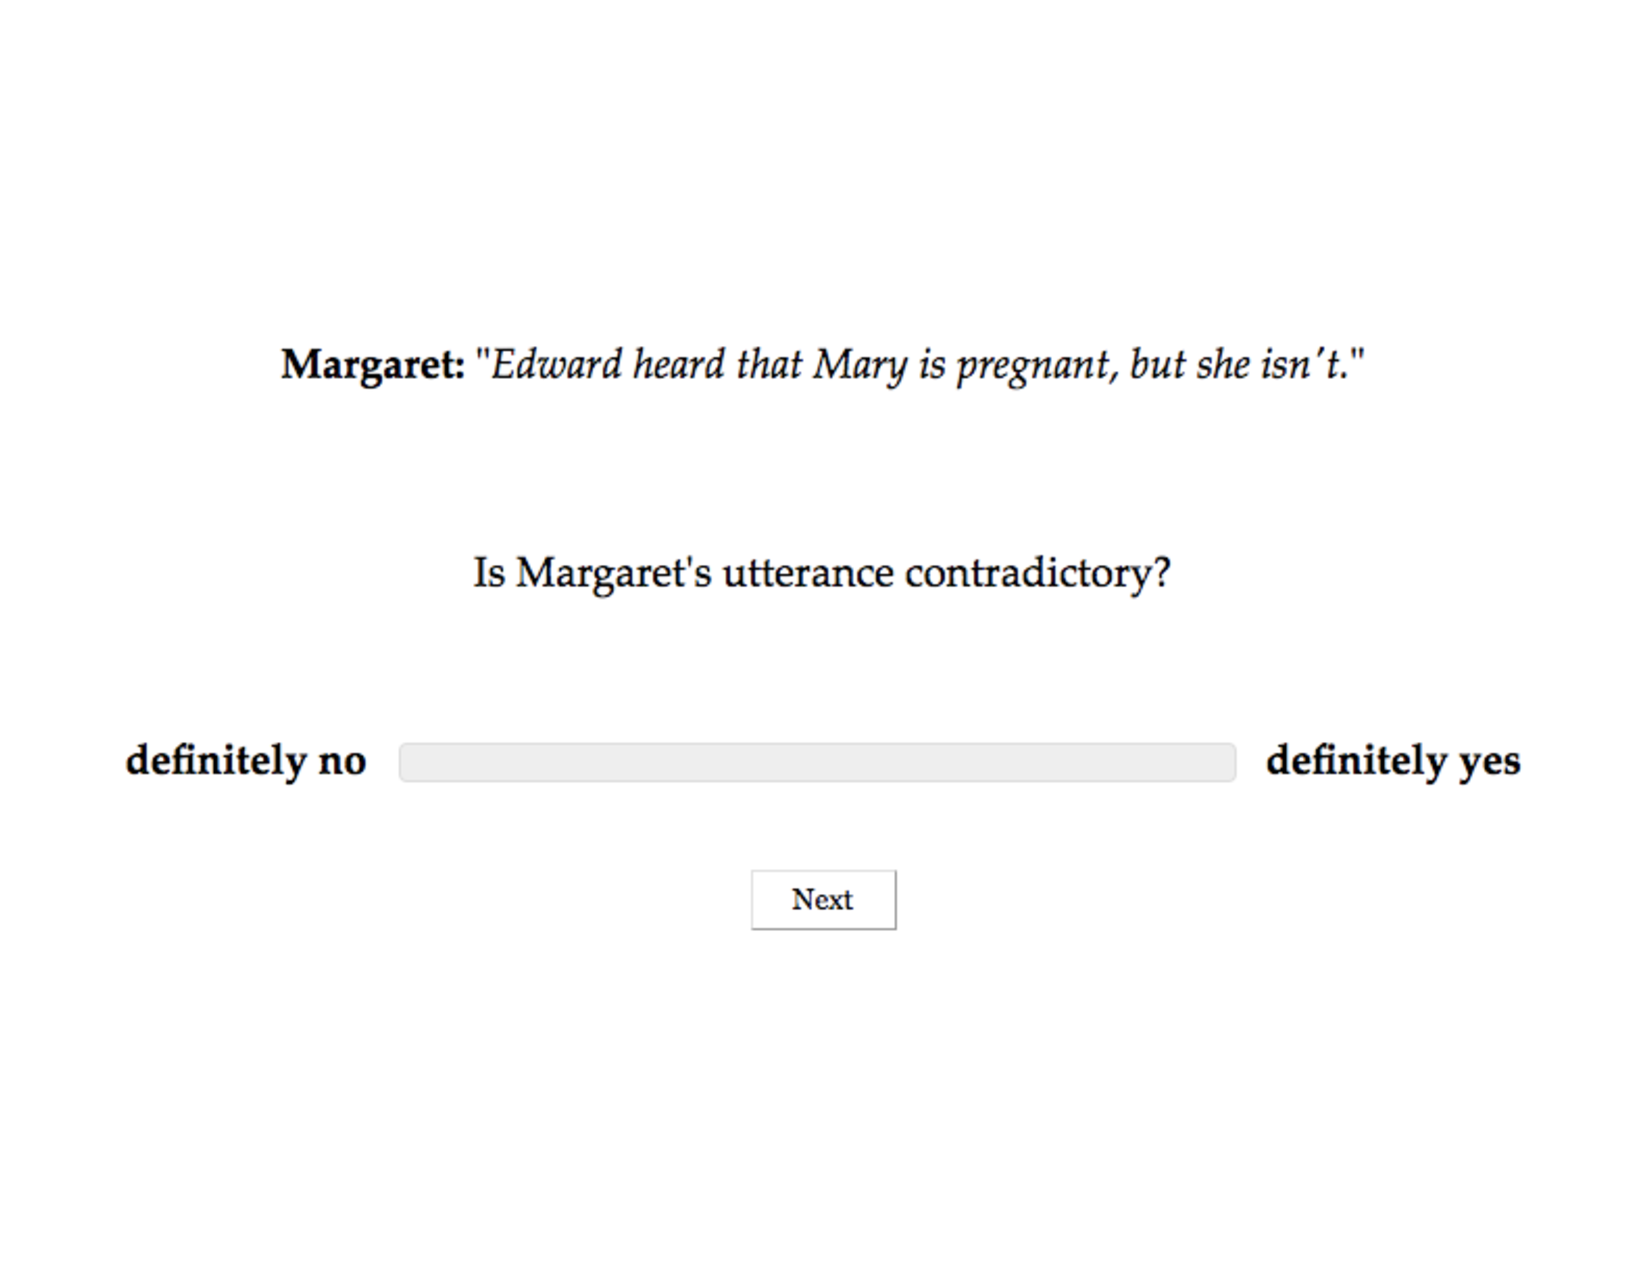
\includegraphics[width=13cm]{figures/contradictory-trial}}
\end{center}
\caption{A sample trial in Experiment 3a}\label{f-trial-exp2}
\end{figure}

To familiarize participants with the task, they first responded to the two familiarization stimuli in (\ref{train}): participants who rated (\ref{train}a) in the lower half of the scale or (\ref{train}b) in the upper half of the scale were given an explanation for why their answer was wrong. Participants could only advance to the 28 stimuli if they gave a plausible rating to the two training stimuli, that is, a rating in the upper half of the scale for (\ref{train}b) and a rating in the lower half for (\ref{train}b).

\begin{exe}
\ex\label{train}
\begin{xlist}
\ex Drew is aware that Patty lives in Canada, but she doesn't.

\ex Drew thinks that Patty lives in Canada, but she doesn't.
\end{xlist}
\end{exe}

After responding to the 28 stimuli, participants filled out a short, optional survey about their age, their gender, their native language(s) and, if English is their native language, whether they are a speaker of American English (as opposed to, e.g., Australian or Indian English). To encourage them to respond truthfully, participants were told that they would be paid no matter what answers they gave in the survey.

\paragraph{Data exclusion}

Prior to analysis, the data from 19 participants who did not self-identify as native speakers of American English were excluded. For the remaining 281 participants, we inspected their responses to the 8 control stimuli: as expected, the group mean rating for the non-contradictory control stimuli in (\ref{control-good}) was at floor (.08)\footnote{The mean contradictoriness rating of the non-contradictory control stimulus that was of the same form as the target stimuli, namely (\ref{control-good}b) {\em Zack believes that I'm married, but I'm actually single}, was higher, at .17, than the mean ratings of the remaining three non-contradictory control stimuli (means: .05 or .06) and identical to that of the target stimuli with {\em think}.}  and the group mean rating for the contradictory control stimuli in (\ref{control-bad}) was at ceiling (.94). This finding shows that, overall, participants attended to and understood the task. The mean ratings of 18 participants were more than 2 standard deviations above the group mean for the non-contradictory control stimuli or below the group mean for the contradictory control stimuli. Closer inspection revealed that these participants' responses to the control stimuli were systematically higher or lower, suggesting that they did not attend to the task or interpreted the task differently. The data from these 18 participants were also excluded. In this experiment, we did not identify any participants who always selected roughly the same point on the response scale. The results presented below are based on data from 263 participants (ages 18-72; median: 36; 126 female, 136 male, 1 other).

\subsubsection{Results and discussion}


Figure \ref{f-veridicality-predicate2} plots the mean contradictoriness ratings for the target and control stimuli. In line with impressionistic judgments reported in the literature, the mean inference ratings for the factive and veridical non-factive predicates are among the highest, and those of the non-factive non-veridical predicates are among the lowest. However, except possibly for {\em be right}, none of the mean contradictoriness ratings are close to those of the contradictory controls.

%   verb              Mean
%   <chr>            <dbl>
% 1 acknowledge     0.672 
% 2 admit           0.711 
% 3 announce        0.448 
% 4 be_annoyed      0.640 
% 5 be_right        0.941 
% 6 confess         0.669 
% 7 confirm         0.767 
% 8 contradictory C 0.960 
% 9 demonstrate     0.720 
%10 discover        0.789 
%11 establish       0.721 
%12 hear            0.238 
%13 inform          0.472 
%14 know            0.838 
%15 non-contrd. C   0.0587
%16 pretend         0.217 
%17 prove           0.858 
%18 reveal          0.634 
%19 say             0.363 
%20 see             0.819 
%21 suggest         0.257 
%22 think           0.171 

\begin{figure}[h!]
\centering

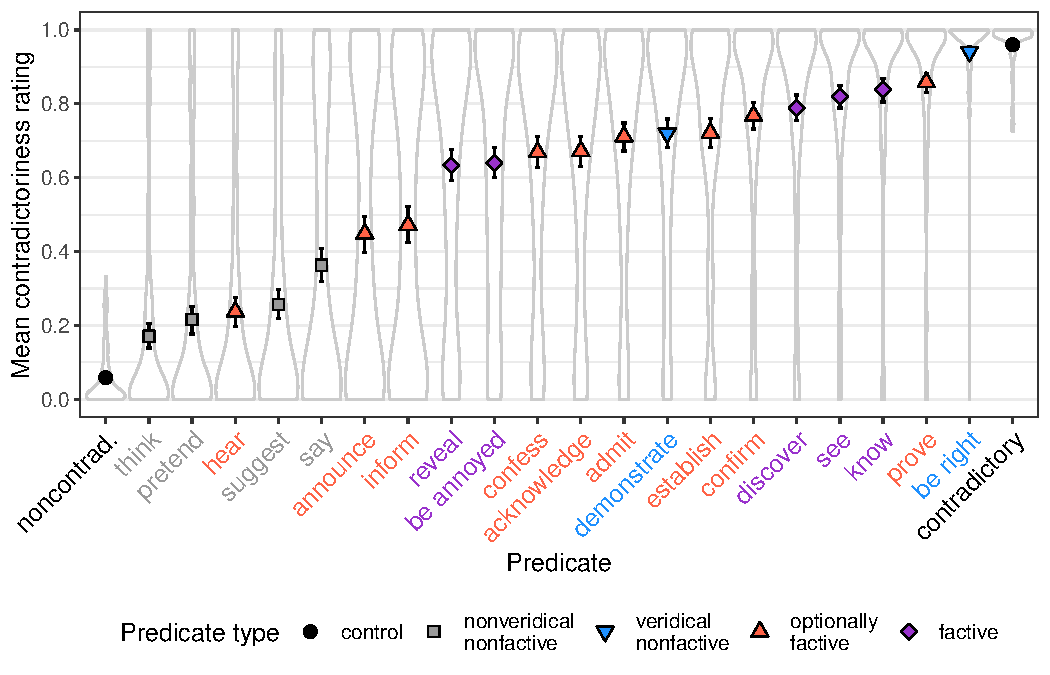
\includegraphics[width=.7\paperwidth]{../../results/2-veridicality2/graphs/means-contradictoriness-by-predicate-variability}

\caption{Mean contradictoriness rating by predicate in Exp.~3a, including the non-contradictory and contradictory controls. Error bars indicate bootstrapped 95\% confidence intervals. Light gray dots indicate individual participants' ratings.}
\label{f-veridicality-predicate2}
\end{figure}

\jd{JD Describe models and connect to text} In other words, none of the contradictoriness ratings for the CCs are statistically indistinguishable from those of the controls with entailed content. This finding suggests that the CCs of none of the 20 predicates are entailed. Consequently, none of the 20 predicates are factive under the definition of factive predicates in (\ref{def}b). 

One may again ask whether the finding of Exp.~3a is an artifact of the gradient response task and whether categorical responses might result in more CCs being classified as entailed. To assess this possibility, we conducted Exp.~3b, which was identical to Exp.~3a but employed a two-alternative forced choice task.

%Contextual factors may influence contradictoriness ratings: for instance, how contradictory an utterance of (\ref{announce3}) is assessed to be may depend on how old or how trustworthy Mary is (see, e.g., \citealt{schlenker10,demarneffe-etal2012}). To allow participants' ratings to reflect degrees of contradictoriness, we collected gradient contradictoriness ratings. We assume that when the content of $\phi$ entails the content of $\psi$, the contradictoriness of an utterance of the form {\em $\phi$ but not $\psi$} is not mitigated by contextual factors, and participants' contradictoriness ratings are at ceiling, that is, indistinguishable from contradictory control stimuli.


\subsection{Exp.~3b: Categorical ratings using the contradictoriness diagnostic for entailment}\label{s32}

\subsubsection{Methods}

\paragraph{Participants} 600 participants with U.S.\ IP addresses and at least 99\% of previous HITs approved were recruited on Amazon's Mechanical Turk platform They were paid \$1 for participating.

\paragraph{Materials and procedure} The materials and procedure were identical to those of Exp.~3a, with the exception of the task: participants responded `yes' or `no' to the question of whether the speaker's utterance is contradictory, as shown in Figure \ref{fig-trial-exp3b}.

\begin{figure}[h!]
\begin{center}
\fbox{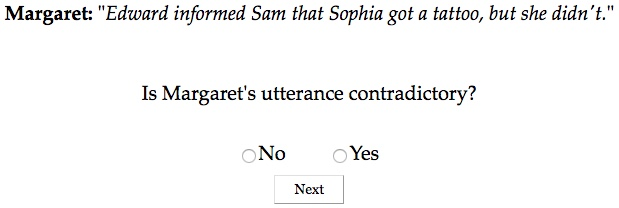
\includegraphics[width=10cm]{figures/Exp3b-trial}}
\end{center}
\caption{A sample trial in Experiment 3b}\label{fig-trial-exp3b}
\end{figure}


\paragraph{Data exclusion} For participants who took the experiment more than once, we only analyzed the data from the first time they took the experiment, leaving data from 430 participants. Prior to analysis, we excluded the data from 30 participants who did not self-identify as native speakers of American English. We also excluded the data from 47 participants who gave more than one wrong rating to one of the eight control sentences, where a wrong ratings was a `yes' to a non-contradictory control and a `no' to a contradictory one. The data from 353 participants (ages 18-73; median: 37; 180 female, 173 male) entered the analysis below. 
    


\subsubsection{Results and discussion}

Figure \ref{fig:3bresults} plots the proportion of `yes' ratings on target and control trials. The findings of Exp.~3b are again very similar to those of Exp.~3a: except possibly for {\em be right}, the contradictoriness ratings for the CCs of none of the predicates are close to the contradictory controls. The Spearman rank correlation between Exps.~3a and 3b is very high, at .985 (see Appendix \ref{a-comparison} for a visualization).

\begin{figure}[h!]
\centering
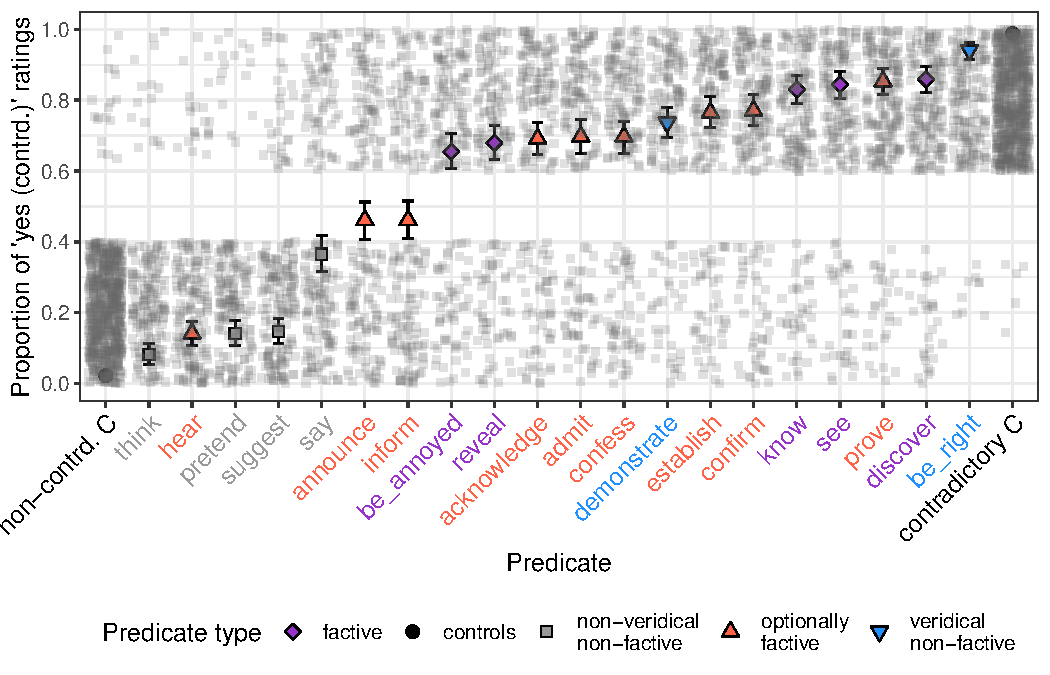
\includegraphics[width=.7\paperwidth]{../../results/6-veridicality2-binary/graphs/proportion-by-predicate-variability-individual}
\caption{Proportion of `yes' ratings by predicate in Exp.~3b. Error bars indicate 95\% bootstrapped confidence intervals. Jittered light gray dots indicate individual participants' ratings of `yes' (coded as 1) and `no' (coded as 0). }
\label{fig:3bresults}
\end{figure}

\jd{insert model info and connect to text} In other words, none of the contradictoriness ratings for the CCs are statistically indistinguishable from those of the controls with entailed content. This finding suggests that the CCs of none of the 20 predicates are entailed. Consequently, as with Exp.~3a, none of the 20 predicates are factive under the definition of factive predicates in (\ref{def}b). 

\subsection{Do projectivity and entailment jointly identify a class of factive predicates?}\label{s33}

According to definition (\ref{def}a), a predicate is factive if and only if its CC is presupposed. As discussed in section \ref{s2}, projection alone does not appear to categorically distinguish factive predicates from optionally factive and non-factive ones and, therefore, fails to identify a class of factive predicates. Definition (\ref{def}b) differs from definition (\ref{def}a) in that a predicate is factive if and only if its CC is not just presupposed but also entailed. In Exps.~2 and 3, we applied two standard diagnostics to the CCs of the 20 clause-embedding predicates: to assess whether the CC of a predicate is entailed, we compared the inference ratings (Exps.~2) and the contradictoriness ratings (Exps.~3) for the CCs to the ratings for control stimuli with entailed content. We assumed that the CC of a predicate is entailed if the ratings for that CC are statistically indistinguishable from these control stimuli, and not entailed if the ratings for that CC are significantly lower. 

Given these assumptions, we found that the CCs of {\em prove, be right, see, discover} and {\em confirm} are entailed based on the gradient and the categorical inference diagnostic (Exps.~2a and 2b), that the CC of {\em know} is entailed based on the categorical inference diagnostic (Exp.~2b) but not on the gradient one (Exp.~2a), and that the CCs of none of the 20 predicates are entailed based on the gradient and categorical contradictoriness diagnostics for entailment (Exps.~3). The differences between the findings of Exps.~2 and 3 suggest that the inference and the contradictoriness diagnostic do not both diagnose entailment, contrary to assumption. Given how widely these diagnostics are used, a pressing question for future research is whether one diagnostic is better suited to diagnosing entailment and how to account for the differences.\footnote{For reasons of space we cannot engage with this question in this paper but only make two observations that are relevant to this question. First, the entailed controls received very high ratings across Exps.~2 and 3, suggesting that all four measures are able to diagnose entailed content. \citet[329]{demarneffe-etal2012} suggested that veridicality ratings are influenced by pragmatic reasoning; see also \citealt{pavlick-kwiatkowski2019}. We agree but consider it unlikely that pragmatic reasoning would only influence participants' ratings on the target stimuli, to the exclusion of the control stimuli. Second, even though ratings for the CCs of the 20 predicates were overall lower with the  contradictoriness diagnostic than the inference diagnostic, the fact that the Spearman rank correlations of the two diagnostics are very high, namely .954 for the two gradient measures and .934 for the two categorical measures, suggests that both are measuring a similar underlying concept.}


Given that the CC of all 20 predicates is at least mildly projective, i.e., presupposed, this means, under the definition of factive predicates in (\ref{def}b), that the predicates {\em prove, be right, see, discover} and {\em confirm} are factive according to the findings of Exp.~2a, that the predicates {\em prove, be right, know, see, discover} and {\em confirm} are factive according to the findings of Exp.~2b, and that none of the 20 predicates are factive according to the findings of Exps.~3. The differences between the findings of Exps.~2 and 3 stand in the way of identifying factive predicates. Moreover, a consequence of the empirical finding that the CCs of more predicates than previously assumed are projective, i.e., presupposed, is that relatively more importance falls to entailment in identifying factive predicates: of all the predicates with projective CCs, those whose CC is entailed are factive and those whose CC is not entailed are not factive. For the 20 predicates we investigated, all of whose CCs are projective, this had the unfortunate consequence that, under the inference diagnostic, the heterogeneous set of predicates {\em prove, be right, see, discover, confirm} and possibly {\em know} are factive and, under the contradictoriness diagnostic, no predicate is factive. In short, considering entailment in the identification of factive predicates does not have the desired effect: the set of factive predicates is either empty or heterogeneous with respect to projection, i.e., not a natural class. We conclude that the definition of factive predicates in (\ref{def}b) fails to identify a class of factive predicates. 

Converging evidence for this conclusion comes from the VerbVeridicality and MegaVeridicality datasets, which both include entailment ratings in addition to the projection ratings discussed in section \ref{s-converging1}. Consider first the VerbVeridicality dataset: in addition to projection ratings for the CCs of the negated variants of the 859 indicative matrix sentences, it also contains entailment ratings for the 859 indicative matrix sentences; an example is given in (\ref{vv-stim-proj2}). 

\begin{exe}
\ex\label{vv-stim-proj2} The GAO has indicated that it is unwilling to compromise.
\end{exe}
To diagnose entailment, three participants rated on a 5-point Likert scale whether the CC is true given the target sentence; one endpoint of the scale was labeled `definitely true' (coded as 2) and the other `definitely not true' (coded as -2). We follow \citet{ross-pavlick2019} in referring to these as `veridicality' ratings. 

Figure \ref{f-vv-projectivity} plots the mean veridicality ratings for the 78 clause-embedding predicates in the VerbVeridicality dataset, with labels for the 15 predicates from our experiments (recall that {\em see} and {\em saw} are plotted separately). On the standard definition of entailment, one would predicates with entailed CCs to have a mean veridicality rating of 2. None of the clause-embedding predicates have a mean veridicality ratings of 2: thus, the CCs of none of these 78 clause-embedding predicates are entailed and, consequently, none of the 78 predicates are factive according to the definition in (\ref{def}b). Relaxing the linking function results in a heterogeneous set of factive predicates: For instance, there are 15 predicates whose CC received a mean veridicality rating at least as high as that of {\em know} (1.5). If one assumes that these CCs are entailed and that CCs with mean projection ratings of at least .3 are presupposed,\footnote{The VerbVeridicality dataset does not include projection ratings for non-projective main clause content to which the projection ratings for the CCs could be compared. The cutoff of a mean projection rating of .3 (for ordinal ratings on a 5-point Likert scale coded from -2 to 2) is therefore arbitrary, though plausible: in our Exp.~1a, for instance, the CC of {\em pretend} was found to be projective compared to the main clause content with a mean certainty rating of .15 (on a scale coded from 0 to 1).} then the set of factive predicates is heterogeneous with respect to projection: it includes {\em notice}, with a mean projection rating of 1.1, {\em give} (1.1), {\em realize} (1.1), {\em explain} (.9) and {\em know} (.8), but also {\em acknowledge} (.5), {\em learn} (.4), {\em saw} (.4) and {\em admit} (.3). In short, on the VerbVeridicality set, too, definition (\ref{def}b) of factive predicates fails to identify a class of factive predicates.

\begin{figure}[H]
\centering
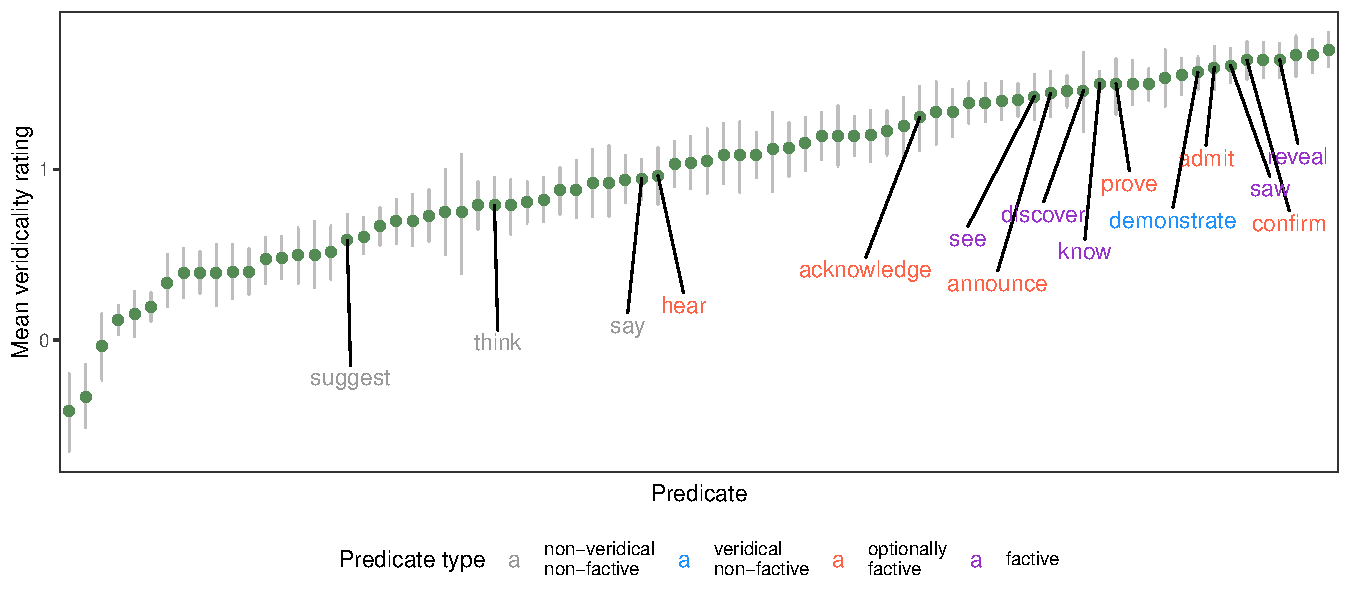
\includegraphics[width=.77\paperwidth]{../../VerbVeridicality-analysis/graphs/means-entailment-by-predicate}

\caption{Mean veridicality rating by predicate in green, with 95\% bootstrapped confidence intervals, for the 78 predicates in the VerbVeridicality dataset (\citealt{ross-pavlick2019}), with labels for the 15 predicates featured in our experiments.}
\label{f-vv-projectivity}
\end{figure}

The MegaVeridicality dataset includes veridicality ratings for the CCs of the same 517 English clause-embedding predicates for which projection ratings were collected. The veridicality ratings were collected for stimuli that combined these predicates with arguments with low lexical content, as shown in (\ref{wr-stim-ent}) for the predicate {\em know}. To diagnose veridicality, participants were asked to respond to the question {\em Did that thing happen?}; the response options were `yes', `maybe or maybe not' and `no'. 

\begin{exe}
\ex\label{wr-stim-ent} Somebody knew that a particular thing happened.
\end{exe}

Each of the 517 predicates in the MegaVeridicality dataset received between 9 and 20 entailment ratings (mean: 10) from 159 participants. To plot the ratings, we coded a `yes' response as 1, a `maybe or maybe not' response as 0 and a `no' response as -1. Figure \ref{f-white-rawlins-ent} plots the mean veridicality ratings for the 517 predicates in the MegaVeridicality dataset, with labels for the 19 predicates from our experiments. On the standard definition of entailment, one would expect predicates with entailed CCs to have a mean veridicality rating of 1. There are 97 clause-embedding predicates that only received `yes'/1 ratings, including 3 of the factive predicates we investigated, namely {\em reveal, know} and {\em be annoyed}; this finding is compatible with the assumption that the CCs of these 97 predicates are entailed.\footnote{\label{mv}It is not clear that the CCs of these 97 predicates are entailed: this set includes {\em inform} (see the discussion in section \ref{s1}) as well as the communication predicates {\em bitch} and {\em howl}, whose CCs are not entailed. For instance, it does not follow from the naturally occurring example with {\em bitch} in (i) that the Democratic party hates all the Jews.

\begin{exe}
\exi{(i)} Rambling to reporters in the Oval Office, Trump bitched that the Democratic party clearly hates all the Jews because of all the support reps Rashida Tlaib and Ilhan Omar received after he strong armed the Israelis into barring them from visiting the country as members of Congress. (\url{https://www.wonkette.com/08-21-2019})
\end{exe}
\citet{white-rawlins-nels2018} assumed that the CCs of 376 of the 517 predicates are entailed because they assumed that the CC of a predicate is entailed if and only if the majority of the responses for a predicate was `yes'. We do not adopt this linking function because it is incompatible with the standard definition of entailment: for instance, given this linking function, the CC of {\em tweet} is entailed because 11 of the 20 participants responded `yes', despite the remaining 9 participants responding `maybe or maybe not'.} If we assume, again, that CCs with mean projection ratings of at least .3 are presupposed, then 92 of the 97 predicates are factive,\footnote{\citet{white-rawlins-nels2018}, who assumed the definition of factive predicates in (\ref{def}b), identified 199 factive predicates in the MegaVeridicality database. However,  this finding is due to the authors assuming that a majority of `yes' responses for a predicate means that the CC is entailed (for positive matrix sentences) or presupposed (for sentences embedded under negation or in a question). As discussed in footnote \ref{mv}, the linking function for entailed CCs is not compatible with the standard definition of entailment. For presupposed CCs, it is not clear that a majority of `yes' responses is motivated as a threshold for projection; see the discussion in section \ref{s22}.} 
 but this set is heterogeneous with respect to projection, including predicates like {\em bother}, with a mean projection rating of .97, {\em inform} (.7), {\em know} (.63), {\em grumble} (.5), {\em notify} (.4), {\em gloat} (.4) {\em convey} (.4) and {\em confirm} (.3). Thus, on the MegaVeridicality set, too, definition (\ref{def}b) fails to identify a class of factive predicates.

\begin{figure}[H]
\centering
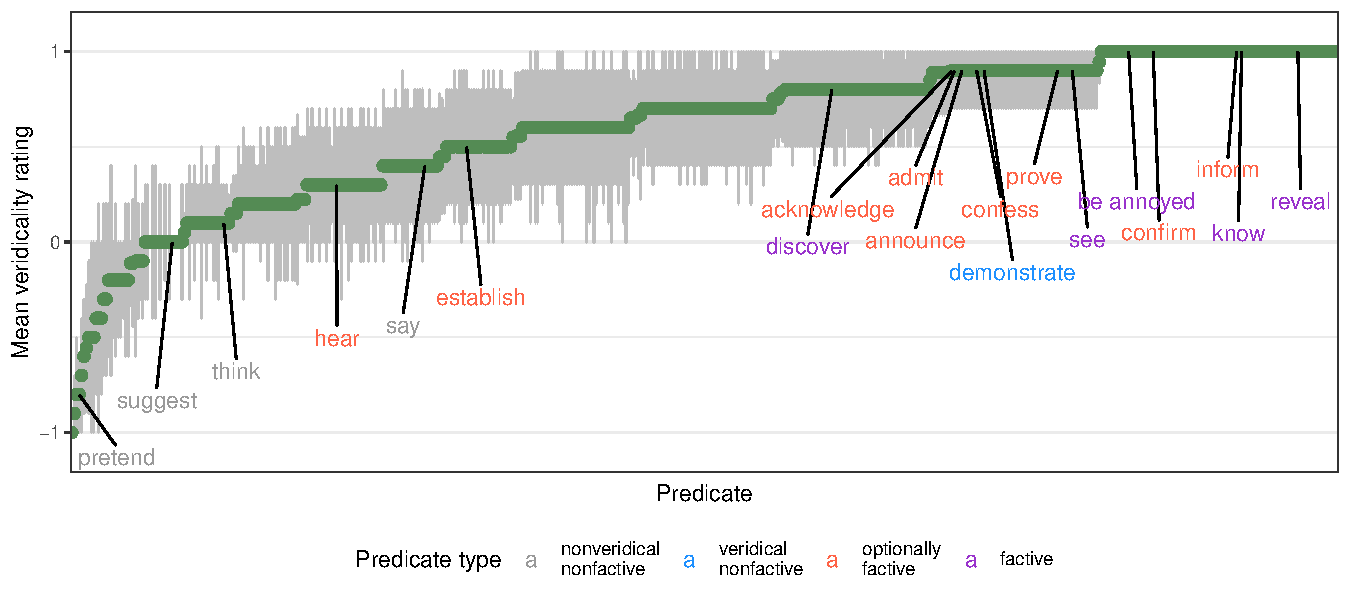
\includegraphics[width=.75\paperwidth]{../../MegaVeridicality-analysis/graphs/means-entailment-by-predicate}

\caption{Mean veridicality rating by predicate in green, with 95\% bootstrapped confidence intervals, for the 517 predicates in the MegaVeridicality dataset (\citealt{white-rawlins-nels2018,white-etal2018b}), with labels for the 19 predicates featured in our experiments.}
\label{f-white-rawlins-ent}
\end{figure}

In sum, contrary to what is expected under the definition of factive predicates in (\ref{def}b), the findings of our Exps.~1, 2 and 3, as well as those of the VerbVeridicality and MegaVeridicality datasets, suggest that projection and entailment of the CC do not jointly identify a class of factive predicates. Depending on how entailment is diagnosed and which linking function is assumed, the set of predicates identified as factive is either empty (if no predicates have entailed CCs) or heterogeneous (because the CCs of more predicates than previously assumed are at least mildly projective, i.e., presupposed, compared to main clause content). 

\section{Discussion}\label{s4}

The question addressed in this paper is: Which predicates are factive? Despite the central role that the distinction between factive and non-factive predicates has played in linguistic theorizing, different answers have been given to this question because, as noted in section \ref{s1}, there is disagreement about how to define factive predicates, uncertainty about whether projection categorically distinguishes factive predicates from optionally factive and non-factive ones, and disagreement about which clause-embedding predicates have entailed CCs. In sections \ref{s2} and \ref{s3}, we presented the findings of experiments designed to investigate which predicates are factive based on  two definitions of factive predicates. Our experiments in section \ref{s2} investigated the definition in (\ref{def}a), according to which a predicate is factive if and only if its CC is presupposed: we found that projection alone does not categorically distinguish factive predicates from optionally factive and non-factive ones and, furthermore, that the CCs of all of the predicates we investigated are at least mildly projective. In section \ref{s3}, we investigated the definition in (\ref{def}b), according to which a predicate is factive if and only if its CC is both presupposed and entailed: our experiments found that, depending on how entailment is diagnosed, there are either no factive predicates or that the set of predicates identified as factive is heterogeneous with respect to projection, i.e., not a natural class. We are therefore led to the conclusion that, at present, there is no empirical evidence for a class of factive predicates that is categorically distinguished from optionally factive and non-factive ones by two properties of the CC, namely projection and entailment. 

One area in which the distinction between factive and non-factive predicates has played a major role is research on projective content. Formal analyses of the projection of the CC of clause-embedding predicates are generally limited to the CCs of factive predicates: the explanandum is assumed to be that the CCs of factive predicates, but not those of optionally factive or non-factive ones, are presuppositions, which may project. On some analyses (e.g., \citealt{heim83,vds92}), factive predicates lexically specify that the CC is required to be entailed by or satisfied in the relevant context; optionally factive and non-factive predicates do not carry such a lexical specification. On other analyses (e.g., \citealt{abrusan2011,abrusan2016,romoli2015,best-question}), projection of the CC is derived from the CC being entailed content that is backgrounded; non-entailed CCs of optionally factive and non-factive predicates are again outside of the scope of these analyses. It is within the context of these formal analyses that we were led to investigate which predicates are factive: we wanted to understand which predicates these analyses apply to. Our conclusion that, at present, there is no empirical evidence for a class of factive predicates is unnerving because it means that it is not clear which predicates these analyses apply to and because it challenges long-held and widespread assumptions about clause-embedding predicates. 

One way forward is to maintain the assumption that there is a class of factive predicates whose CCs are distinct from those of optionally factive and non-factive predicates and to continue to search for an empirical diagnostic of factive predicates. Another way forward, and the one we advocate for, is to embrace the our findings: the CCs of many more clause-embedding predicates than previously assumed are projective, there is a lot of variability in how projective the CCs are, and whether the CC is entailed is irrelevant to understanding projection. These findings, we argue, point to several exciting avenues for future research. 

First, the finding that the CCs of more clause-embedding predicates than previously assumed are projective means that research on projective content has a much broader empirical scope than previously assumed. Given that research on projective content has focused almost entirely on the the CCs of purportedly factive predicates, to the exclusion of the CCs of optionally factive and non-factive ones, our finding means that we are now tasked with investigating and formally analyzing the projectivity of the CCs of a much broader set of clause-embedding predicates than before. One approach to predicting the projectivity of the CCs of optionally factive and non-factive predicates has been to assume that such predicates are ambiguous: \citet{spector-egre2015}, for instance, proposed (p.1736) that predicates like {\em tell, predict} and {\em announce}  have a factive lexical entry on which the CC is entailed and presupposed and a non-factive one on which it is not. The findings of our Exps.~1 point to some difficulties for this approach. For one, this approach requires the assumption of widespread ambiguity among clause-embedding predicates. It is also not clear which predicates would only have a factive or only a non-factive lexical entry, and which ones would be ambiguous. And, finally, the approach cannot account for the observed by-predicate projection variability: for instance, the assumption that both {\em discover} and {\em announce} have a factive and a non-factive lexical entry does not predict that the CC of {\em discover} more projective than the CC of {\em announce}. 

A second avenue for future research emerges from the observation that there is a lot of variability in how projective the CCs of clause-embedding predicates are. Research on projective content has identified a number of factors that influence the projectivity of utterance content, including context, lexical content, prior content probability, at-issueness, information structure and the perceived degree of reliability and trustworthiness of the attitude holder (e.g., \citealt{gazdar79a,gazdar79b,beaver-belly,schlenker10,brst-salt10,best-question,abrusan2011,abrusan2016,anand-hacquard2014,cummins-rohde2015,djaerv-bacovcin-salt27,tonhauser-salt26,tonhauser-guarani-variability,tbd-variability,tonhauser-etal-sub23}). An exciting question for future research is whether these factors are implicated in the projectivity of the CCs of all clause-embedding predicates, or only particular subsets, and whether they contribute to the observed projection variability. 

One of the factors that clearly plays a role in predicting projection variability is the lexical meaning of the clause embedding predicate: as shown by our Exps.~1, as well as in \citealt{tbd-variability}, a binary distinction between factive and non-factive predicates, or a ternary distinction between factive, optionally factive and non-factive predicates, is too coarse to predict the observed projection variability. We hypothesize that more fine-grained distinctions that are based on the lexical meaning and discourse use of clause-embedding predicates are critical to understanding the projectivity of the CC and we also hypothesize that the CCs of classes of predicates that share lexical meanings and discourse uses are similar in projectivity. 

We are aware of two tentative proposals along those lines in the recent literature. \citet{anand-hacquard2014} hypothesized that listeners may take speakers to be committed to the CC of assertive predicates, like {\em acknowledge, admit} and {\em confirm},  ``because of the kind of discourse moves that these predicates report'' (p.74). Specifically, utterances of sentences with these predicates can be used to report the success of an uptake in a reported common ground: for example, an utterance of a sentence like {\em Kim confirmed that Mary is the murderer} can report that the content $p$ of the  complement, that Mary is the murderer, is accepted ``into the common ground of the reported discourse'' ({\em ibid.}). The authors suggested that ``[t]his acceptance of $p$ can easily bleed into the actual common ground, under the assumption that no subsequent move removed $p$ from the common ground'' (p.74f). \citet{karttunen2016}  proposed different paths to projection for different classes of clause-embedding predicates. For instance, for predicates with {\em that-}clause subjects that do not involve an attitude holder, like {\em be odd, be tragic} or {\em count}, the projection of the CC is derived from its status as a presupposition; with predicates that express a propositional attitude, like {\em know} or {\em forget}, the speaker is only necessarily committed to the attitude holder being committed to the truth of the CC and speaker commitment to the CC is derived as a generalized conversational implicature; for a third subclass of change-of-state predicates, including {\em discover} and {\em notice}, the CC is entailed but its projection is derived pragmatically; and for a fourth subclass of communicative predicates, like {\em acknowledge, admit} and {\em confess}, the speaker is merely committed to the attitude holder having communicated something that the attitude holder wishes to present as a fact. While such proposals need to be fleshed out in more detail to be predictive, we believe that detailed analyses of the lexical meanings of clause-embedding predicates are a fruitful path to a better understanding of the projection of their CCs.


%A second proposal was sketched in \citealt{karttunen2016}: this work gave up on the idea that there is a class of factive predicates with a uniform definition and instead proposed that more fine-grained distinctions among clause-embedding predicates play a role in the projection of the CC. \citet{karttunen2016} distinguished several subclasses of factive predicates: for instance, for predicates with {\em that-}clause subjects that do not involve an attitude holder, like {\em be odd, be tragic} or {\em count}, the projection of the CC is derived from its status as a presupposition; with predicates that express a propositional attitude, like {\em know} or {\em forget}, the speaker is only necessarily committed to the attitude holder being committed to the truth of the CC and speaker commitment to the CC is derived as a generalized conversational implicature; for a third subclass of change-of-state predicates, including {\em discover} and {\em notice}, the CC is entailed but its projection is derived pragmatically; and for a fourth subclass of communicative predicates, like {\em acknowledge, admit} and {\em confess}, the speaker is merely committed to the attitude holder having communicated something that the attitude holder wishes to present as a fact. While \citepos{karttunen2016} proposal, too, would need to be fleshed out in more detail to be predictive, we believe that detailed analyses of the lexical meanings of clause-embedding predicates are a fruitful path to a better understanding of the projection of their CCs.


%One attempt is presented in \citealt{schlenker10}, who proposed that {\em announce} is a ``part-time presupposition trigger'' (p.139): ``in some contexts, [{\em announce}, JT\&JD] does not entail the truth of its complement; in other contexts, it entails and {\em presupposes} the truth of the complement'' ({\em ibid.}). The notion of entailment adopted by Schlenker appears to be a context-dependent one, not the standard notion assumed here. We refer to his notion as `Schlenker-entailment': in context $c$, the content of sentence $\phi$ Schlenker-entails the content of sentence $\psi$ if and only the truth of $\psi$ follows from the truth of $\phi$ in $c$.  Thus, on Schlenker's proposal, a context in which the CC of {\em announce} projects is a context in which a true assertion of the unembedded sentence with {\em announce} Schlenker-entails the content. Abstracting over contexts, it follows that if the CC of {\em announce} is less projective than that of some other clause-embedding predicate $P$, we expect the CC of {\em announce} to follow less strongly from true assertions of unembedded sentences with {\em announce} than from such assertions with $P$. This expectation is not borne out: the CC of {\em announce} is less projective than that of {\em hear} (Exp.~1), but on both the inference diagnostic (Exp.~2a) and the contradictoriness diagnostic (Exp.~3a), the CC of {\em announce} received significantly higher responses than that of {\em hear}. We conclude that the findings of our experiments are not predicted by \citetpos{schlenker10} proposal for the projectivity of the CC of non-factive predicates like {\em announce}.

\section{Conclusions}\label{s5}

Linguistic research since \citealt{kiparsky-kiparsky70} has assumed that properties of the content of the clausal complement distinguish factive predicates from non-factive and (what we call) optionally factive ones. This paper investigated whether the content of the complement of 20 English clause-embedding predicates is projective and entailed, with the goal of identifying factive predicates according to two definitions found in the literature. Our experiments revealed that projection alone does not categorically distinguish factive predicates from optionally factive and non-factive ones, and that a class of factive predicates also does not emerge from the additional consideration of entailment, as assessed by two standard diagnostics. We concluded that there is, at present, no empirical support for the assumed categorical distinction between factive predicates, on the one hand, and optionally factive and non-factive ones, on the other. This finding calls for a reassessment of projection analyses that are limited to the content of the complement of factive predicates, and also opens up several exciting new avenues for empirical and theoretical research on the projection of the contents of the complements of clause-embedding predicates.




\appendix

\setcounter{table}{0}
\renewcommand{\thetable}{A\arabic{table}}

\setcounter{figure}{0}
\renewcommand{\thefigure}{A\arabic{figure}}

%\section{Citations}
%
%That both properties are ascribed to presuppositions, including the CC of factive predicates, can be seen from the following quotes:
%
%\begin{itemize}[topsep=0pt,itemsep=-3pt,leftmargin=12pt]
%
%\item \citealt[66f.]{beaver01}: \citet[119-123]{gazdar79a} ``describes the inferences associated with factive verbs, definite descriptions, aspectual verbs, and clefts as being indefeasible in simple affirmative sentences'', that is, ``entailments''.
%
%\item \citealt[355]{ccmg90}: ``A sentence can both entail and presuppose another sentence [...]. Thus, [{\em Joan realizes that syntax deals with sentence structure}] both entails and presupposes [{\em Syntax deals with sentence struture}]."
%
%\item \citealt[345]{vds92}: ``Note that [global accommodation, that is, projectivity, JT\&JD] is what we would expect given the intuitive notion of presupposition as information taken for granted and note also that this explains the intuition that presuppositions [...] are entailed by their matrix sentence.''
%
%\item \citealt[3]{abbott06}: ``we will need to be careful to distinguish entailments that are presupposed from what I will call ``ordinary, simple entailments'', which are not also presuppositions.''
%
%\item \citealt[139]{schlenker10}: ``we obtain the pattern of inference which is characteristic of presuppositions: an entailment of the positive sentence is preserved under negation and in questions''
%
%
%\item \citealt[77]{anand-hacquard2014}: ``we will adopt the pragmatic view of presupposition triggering, according to which presuppositions are lexical entailments that are backgrounded based on pragmatic principles"
%
%\item {\bf \citealt[fn.7]{spector-egre2015}: Assuming that any presupposition of a sentence is also an entailment of this sentence, it follows that a predicate that is factive with respect to its declarative complement is always also veridical with respect to its declarative complement.}
%
%\end{itemize}

\section{20 complement clauses}\label{a-clauses}

The following clauses realized the complements of the predicates in the three experiments: 

\begin{enumerate}[leftmargin=3ex,itemsep=-2pt]

\begin{multicols}{2}

\item Mary is pregnant.
\item Josie went on vacation to France.
\item Emma studied on Saturday morning.
\item Olivia sleeps until noon.
\item Sophia got a tattoo.
\item Mia drank 2 cocktails last night.
\item Isabella ate a steak on Sunday.
\item  Emily bought a car yesterday.
\item  Grace visited her sister.
\item Zoe calculated the tip.

\columnbreak

\item  Danny ate the last cupcake.
\item  Frank got a cat.
\item  Jackson ran 10 miles.
\item  Jayden rented a car.
\item  Tony had a drink last night.
\item  Josh learned to ride a bike yesterday.
\item  Owen shoveled snow last winter.
\item  Julian dances salsa.
\item  Jon walks to work.
\item  Charley speaks Spanish.

\end{multicols}

\end{enumerate}

\section{Details on the Bayesian models for Experiments 1a, 2a, and 3a}\label{modeldetails}

This appendix provides details on the data analysis conducted for Exps.~1a, 2a, and 3a. We first motivate the use of Beta regression rather than linear regression. We then provide a brief primer on how to interpret Bayesian mixed effects Beta regression models. We then report the model output for the three experiments.

\subsection{Motivation for using Bayesian mixed effects Beta regression}

There are three separate pieces to motivate: the use of \emph{mixed effects}, the use of a \emph{Bayesian} rather than \emph{frequentist} models, and the use of \emph{Beta regression} rather than \emph{linear regression}. 

\textbf{Using mixed effects} refers to the practice of modeling the outcome variable, here slider ratings, as a function of not just fixed effects of interest (i.e., predicate) but also as the result of possible random variability that is not of theoretical interest (e.g., random by-participant or by-item variability). This is standard practice in psycholinguistic studies and allows the researcher to trust that any observed effects of theoretical interest are true average effects rather than the result of idiosyncratic behavior (e.g., of participants or items). This is also the motivation for using mixed effects in Exps.~1b, 2b, and 3b.

\textbf{Using Bayesian models} rather than frequentist models is increasingly becoming the norm in psycholinguistic studies as computational power has increased and running Bayesian models has become more accessible with the introduction of R packages such as \verb|brms| \citep{buerkner2017}. The presence of an effect in frequentist models is evaluated by checking whether the {\em p-}value is smaller than $.05$, where the {\em p-}value is defined as the probability of obtaining data that is as skewed or more skewed than the observed data if the null-hypothesis was true, i.e., if the hypothesized effect was absent. Parameter estimates in frequentist models are obtained via maximum-likelihood techniques, i.e., by estimating the parameter values that maximize the probability of observing the data. Bayesian models, by contrast, return a full posterior distribution over parameter values that take into account not just the probability of the data under the parameter values, but also the prior probability of parameter values. In order to evaluate the evidence for an effect of a predictor of interest, one can report 95\% credible intervals and the posterior probability $P(\beta < 0)$ or $P(\beta > 0)$ that the predictor coefficient $\beta$ is either lower or greater than zero, depending on the direction of the expected effect. A 95\% credible interval (CI) demarcates the range of values that comprise 95\% of probability mass of the posterior beliefs such that no value inside the CI has a lower probability than any point outside it \citep{Jaynes1976, Morey2016}. There is substantial evidence for an effect if zero is (by a reasonably clear margin) not included in the 95\% CI and $P(\beta > 0)$ or $P(\beta < 0)$ is close to zero or one. Posterior probabilities indicate the probability that the parameter has a certain value, given the data and model -- these probabilities are thus \emph{not} frequentist {\em p-}values. In order to present statistics as close to widely used frequentist practices, and following \citealt{Nicenboim2016}, we defined an inferential criterion that seems familiar (95\%), but the strength of evidence should not be taken as having clear cut-off points (such as in a null-hypothesis significance testing framework).

\textbf{Using Beta regression} rather than linear regression was motivated by the violation of two of the  assumptions of linear regression: first, that residuals be normally distributed (where ``residuals'' refers to the residual error for each data point after fitting the model), and second, that the error term exhibit homoscedasticity (that it be roughly the same across different conditions). Slider ratings data has the property of being bounded by its endpoints (which we code as 0 and 1, respectively). This often leads to ``bunching'' behavior at the endpoints (see Figure \ref{app:bunch} \jd{insert} for the distribution of raw ratings in Exp.~1a). This, in turn, can lead to the violation of both of the above assumptions. Intuitively, this is because conditions that elicit ratings closer to endpoints necessarily have a compressed variance; consequently, a condition's mean and its variance are not independent. Beta regression is useful here because it allows for modeling an arbitrarily distributed outcome variable in the $[$0,1$]$ interval. The Beta distribution is characterized by two parameters, one capturing the mean $\mu$ of the distribution and one capturing its precision $\phi$, a measure of dispersion. The greater the precision, the more concentrated the values are around the mean, i.e., the lower the variance of the distribution.  We follow \citet{smithson2006} in modeling $\mu$ and $\phi$ separately for each predictor. That is, we allow each predictor to affect both the mean and the precision of the outcome variable's distribution. 

\subsection{Coding choices and interpreting model output}

Because the outcome variable contained the values 0 and 1, which Beta regression is undefined for, we applied a common transformation to ratings before the main analysis that rescales values $y$ to fall in the open unit interval (0,1)  \citep{smithson2006}. First, we apply $y' = (y-a)/(b-a)$, where $b$ is the highest possible slider rating and $a$ is the smallest possible slider rating. The range is then compressed to not include 0 and 1 by applying $y'' = [y'(N-1) + 1/2]/N$, where $N$ is the total number of observations.

The $\mu$ parameter is modeled via a logit link function (default for Beta regression in \verb|brms|), though other links that squeeze $\mu$ into the $[$0,1$]$ interval are possible. The $\phi$ is modeled via a log link, which ensures that values of $\phi$ are strictly positive, which is necessary because a variance cannot be negative. 

We allowed both $\mu$ and $\phi$ to vary as a function of predicate, with reference level set to main clause control (Exp.~1a), entailing control (Exp.~2a), and contradictory control (Exp.~3a), respectively. We also allowed random intercept adjustments to each parameter by participant and by item, where item was defined as a unique combination of a predicate and a complement clause. Four chains converged after 2000 iterations each (warmup = 1000, \(\hat{R}=1\) for all estimated parameters) with a target acceptance rate of .95 and a maximum treedepth of 15.

Table \ref{tab:exp1amodelresults} shows the posterior estimates of $\mu$ and $\phi$ with their 95\% credible intervals.

\jd{CONTINUE HERE}

%\item The model provided evidence for the predicted effect of the at-issueness of the generalization on the at-issueness of the prejacent: the prejacent of EASs for which the truth of the generalizations was more likely to follow from the common ground were more likely to receive a `yes' (at-issue) rating than the prejacent of EAS for which the truth of the generalization was less likely to follow from the common ground  (posterior mean $\beta$ = 1.29, 95\% CI={[}0.69,1.87{]}, $P(\beta > 0)$ = 1). This finding suggests that the prejacent of EASs is more at-issue when the generalization is less at-issue than when the generalization is more at-issue, as predicted by the analysis in section \ref{s2}.

\begin{table}
\caption{Maximum a posteriori (MAP) model estimates for projection ratings from Exp.~1a (left and middle column, mean $\mu$ and precision $\phi$) and Exp.~1b (right column, $\beta$)  with 95\% credible intervals. Contrast of each predicate is with main clause control reference level. MAP estimates for which there is no evidence that they are different from 0 are italicized.}
\small
\begin{center}
\begin{tabular}{l c c c}
\toprule
& \multicolumn{2}{c}{Exp.~1a: Beta regression} & Exp.~1b: logistic regression \\
Predictor & Estimated $\mu$ & Estimated $\phi$ & Estimated $\beta$\\
\midrule
\multirow{2}{*}{Intercept} & $-1.88 $  & $1.16 $ & $-6.37 $       \\
& $[-1.98;\ -1.78]$ & $[1.02;\ 1.29]$  & $[-7.10;\ -5.72]$ \\
[.25em]
\multirow{2}{*}{acknowledge} & $2.62 $ & $-0.67 $  & $8.00 $        \\
& $[2.45;\ 2.80]$  & $[-0.86;\ -0.49]$ & $[7.31;\ 8.78]$   \\
[.25em]
\multirow{2}{*}{admit} & $2.45 $ & $-0.65 $  & $7.29 $        \\
& $[2.29;\ 2.61]$  & $[-0.83;\ -0.48]$ & $[6.60;\ 8.04]$   \\
[.25em]
\multirow{2}{*}{announce}  & $2.14 $ & $-0.74 $  & $6.70 $        \\
& $[1.98;\ 2.30]$  & $[-0.92;\ -0.57]$ & $[6.04;\ 7.45]$   \\
[.25em]
\multirow{2}{*}{be annoyed} & $3.56 $ & $-0.30 $  & $9.41 $        \\
& $[3.37;\ 3.75]$  & $[-0.51;\ -0.10]$ & $[8.64;\ 10.22]$  \\
[.25em]
\multirow{2}{*}{be right} & $0.52 $ & $-0.21 $  & $2.33 $        \\
& $[0.36;\ 0.68]$  & $[-0.40;\ -0.01]$ & $[1.50;\ 3.21]$   \\
[.25em]
\multirow{2}{*}{confess} & $2.29 $ & $-0.71 $  & $6.75 $        \\
& $[2.13;\ 2.45]$  & $[-0.88;\ -0.54]$ & $[6.07;\ 7.50]$   \\
[.25em]
\multirow{2}{*}{confirm} & $1.31 $ & $-0.46 $  & $4.27 $        \\
& $[1.15;\ 1.46]$  & $[-0.64;\ -0.28]$ & $[3.60;\ 5.01]$   \\
[.25em]
\multirow{2}{*}{demonstrate} & $1.78 $ & $-0.59 $  & $5.31 $        \\
& $[1.63;\ 1.93]$  & $[-0.76;\ -0.41]$ & $[4.64;\ 6.06]$   \\
[.25em]
\multirow{2}{*}{discover}  & $2.90 $ & $-0.67 $  & $8.46 $        \\
& $[2.72;\ 3.07]$  & $[-0.85;\ -0.48]$ & $[7.75;\ 9.25]$   \\
[.25em]
\multirow{2}{*}{establish} & $1.42 $ & $-0.55 $  & $4.51 $        \\
& $[1.26;\ 1.58]$  & $[-0.73;\ -0.38]$ & $[3.83;\ 5.26]$   \\
[.25em]
\multirow{2}{*}{hear}  & $2.71 $ & $-0.79 $  & $8.22 $        \\
& $[2.53;\ 2.88]$  & $[-0.98;\ -0.61]$ & $[7.50;\ 9.01]$   \\
[.25em]
\multirow{2}{*}{inform}  & $3.00 $ & $-0.60 $  & $9.13 $        \\
& $[2.82;\ 3.18]$  & $[-0.79;\ -0.41]$ & $[8.38;\ 9.94]$   \\
[.25em]
\multirow{2}{*}{know}  & $3.37 $ & $-0.49 $  & $9.72 $        \\
& $[3.18;\ 3.56]$  & $[-0.70;\ -0.29]$ & $[8.94;\ 10.57]$  \\
[.25em]
\multirow{2}{*}{pretend} & $0.32 $ & $-0.19 $  & $3.22 $        \\
& $[0.15;\ 0.49]$  & $[-0.38;\ -0.00]$ & $[2.50;\ 4.03]$   \\
[.25em]
\multirow{2}{*}{prove} & $1.16 $ & $-0.21 $  & $3.92 $        \\
& $[1.01;\ 1.31]$  & $[-0.40;\ -0.03]$ & $[3.21;\ 4.67]$   \\
[.25em]
\multirow{2}{*}{reveal}  & $2.59 $ & $-0.72 $  & $7.41 $        \\
& $[2.42;\ 2.76]$  & $[-0.90;\ -0.55]$ & $[6.72;\ 8.16]$   \\
[.25em]
\multirow{2}{*}{say} & $0.78 $ & \emph{-0.12}  & $3.10 $        \\
& $[0.63;\ 0.93]$  & $[-0.30;\ 0.06]$ & $[2.35;\ 3.93]$   \\
[.25em]
\multirow{2}{*}{see} & $3.01 $ & $-0.70 $  & $8.74 $        \\
& $[2.83;\ 3.19]$  & $[-0.90;\ -0.51]$ & $[8.03;\ 9.55]$   \\
[.25em]
\multirow{2}{*}{suggest} & $0.79 $ & \emph{-0.17}  & $3.22 $        \\
& $[0.63;\ 0.94]$  & $[-0.36;\ 0.02]$ & $[2.49;\ 3.99]$   \\
[.25em]
\multirow{2}{*}{think} & $0.62 $ & \emph{0.01} & $2.54 $        \\
& $[0.47;\ 0.78]$  & $[-0.17;\ 0.20]$ & $[1.75;\ 3.40]$   \\
\bottomrule
\end{tabular}
\label{tab:exp1amodelresults}
\end{center}
\end{table}

\normalsize

\section{Details on the Bayesian models for Experiments 1b, 2b, and 3b}\label{modeldetails-b}

\subsection{Model output of Exp.~1b}

Formula: \tiny \verb|model.brms.proj.b = brm(nResponse ~ verb + (1/workerid) + (1/item), data=cd, family=bernoulli(), cores = 4, control=list(max_treedepth = 15))| \normalsize

\begin{table}
\begin{center}
\begin{tabular}{l c }
\hline
 & Model 1 \\
\hline
b\_Intercept       & $-6.37^{*}$       \\
                   & $[-7.10;\ -5.72]$ \\
be\_right   & $2.33^{*}$        \\
                   & $[1.50;\ 3.21]$   \\
think       & $2.54^{*}$        \\
                   & $[1.75;\ 3.40]$   \\
say         & $3.10^{*}$        \\
                   & $[2.35;\ 3.93]$   \\
pretend     & $3.22^{*}$        \\
                   & $[2.50;\ 4.03]$   \\
suggest     & $3.22^{*}$        \\
                   & $[2.49;\ 3.99]$   \\
prove       & $3.92^{*}$        \\
                   & $[3.21;\ 4.67]$   \\
confirm     & $4.27^{*}$        \\
                   & $[3.60;\ 5.01]$   \\
establish   & $4.51^{*}$        \\
                   & $[3.83;\ 5.26]$   \\
demonstrate & $5.31^{*}$        \\
                   & $[4.64;\ 6.06]$   \\
announce    & $6.70^{*}$        \\
                   & $[6.04;\ 7.45]$   \\
confess     & $6.75^{*}$        \\
                   & $[6.07;\ 7.50]$   \\
admit       & $7.29^{*}$        \\
                   & $[6.60;\ 8.04]$   \\
reveal      & $7.41^{*}$        \\
                   & $[6.72;\ 8.16]$   \\
acknowledge & $8.00^{*}$        \\
                   & $[7.31;\ 8.78]$   \\
hear        & $8.22^{*}$        \\
                   & $[7.50;\ 9.01]$   \\
discover    & $8.46^{*}$        \\
                   & $[7.75;\ 9.25]$   \\
see         & $8.74^{*}$        \\
                   & $[8.03;\ 9.55]$   \\
inform      & $9.13^{*}$        \\
                   & $[8.38;\ 9.94]$   \\
be\_annoyed & $9.41^{*}$        \\
                   & $[8.64;\ 10.22]$  \\
know        & $9.72^{*}$        \\
                   & $[8.94;\ 10.57]$  \\
\hline
\multicolumn{2}{l}{\scriptsize{$^*$ 0 outside 95\% credible interval}}
\end{tabular}
\caption{Model output of Exp.~1b}
\label{table:coefficients1b}
\end{center}
\end{table}

\subsection{Model output of Exp.~2b}

Formula: \tiny \verb|model.brms.proj.b = brm(nResponse ~ verb + (1/workerid) + (1/item), data=cd, family=bernoulli(), cores = 4, control=list(max_treedepth = 15,adapt_delta=.95))| \normalsize

\begin{table}
\begin{center}
\begin{tabular}{l c }
\hline
 & Model 1 \\
\hline
b\_Intercept       & $6.20^{*}$          \\
                   & $[5.52;\ 6.98]$     \\
acknowledge & $-1.58^{*}$         \\
                   & $[-2.47;\ -0.70]$   \\
admit       & $-1.83^{*}$         \\
                   & $[-2.72;\ -0.97]$   \\
announce    & $-4.39^{*}$         \\
                   & $[-5.17;\ -3.68]$   \\
be\_annoyed & $-1.36^{*}$         \\
                   & $[-2.31;\ -0.46]$   \\
be\_right   & $0.36$              \\
                   & $[-0.93;\ 1.89]$    \\
confess     & $-2.79^{*}$         \\
                   & $[-3.60;\ -2.04]$   \\
confirm     & $-0.85$             \\
                   & $[-1.84;\ 0.14]$    \\
demonstrate & $-3.35^{*}$         \\
                   & $[-4.15;\ -2.63]$   \\
discover    & $-0.50$             \\
                   & $[-1.57;\ 0.64]$    \\
establish   & $-1.92^{*}$         \\
                   & $[-2.76;\ -1.12]$   \\
hear        & $-7.57^{*}$         \\
                   & $[-8.41;\ -6.84]$   \\
inform      & $-3.93^{*}$         \\
                   & $[-4.71;\ -3.22]$   \\
know        & $-0.27$             \\
                   & $[-1.39;\ 0.96]$    \\
nonMent.C   & $-11.92^{*}$        \\
                   & $[-12.94;\ -11.01]$ \\
pretend     & $-10.78^{*}$        \\
                   & $[-11.83;\ -9.85]$  \\
prove       & $0.92$              \\
                   & $[-0.57;\ 2.91]$    \\
reveal      & $-2.37^{*}$         \\
                   & $[-3.21;\ -1.54]$   \\
say         & $-5.79^{*}$         \\
                   & $[-6.59;\ -5.09]$   \\
see         & $-0.49$             \\
                   & $[-1.51;\ 0.62]$    \\
suggest     & $-8.75^{*}$         \\
                   & $[-9.62;\ -7.95]$   \\
think       & $-9.71^{*}$         \\
                   & $[-10.65;\ -8.87]$  \\
\hline
\multicolumn{2}{l}{\scriptsize{$^*$ 0 outside 95\% credible interval}}
\end{tabular}
\caption{Model output of Exp.~2b}
\label{table:coefficients}
\end{center}
\end{table}

\subsection{Model output of Exp.~3b}

Formula: \tiny \verb|model.brms.proj.b = brm(nResponse ~ verb + (1/workerid) + (1/item), data=cd, family=bernoulli(), cores = 4, control=list(max_treedepth = 15,adapt_delta=.95))| \normalsize


\begin{table}
\begin{center}
\begin{tabular}{l c }
\hline
 & Model 1 \\
\hline
b\_Intercept        & $6.17^{*}$          \\
                    & $[5.55;\ 6.88]$     \\
acknowledge  & $-4.89^{*}$         \\
                    & $[-5.65;\ -4.21]$   \\
admit        & $-4.86^{*}$         \\
                    & $[-5.59;\ -4.19]$   \\
announce     & $-6.46^{*}$         \\
                    & $[-7.20;\ -5.80]$   \\
be\_annoyed  & $-5.18^{*}$         \\
                    & $[-5.91;\ -4.51]$   \\
be\_right    & $-1.90^{*}$         \\
                    & $[-2.70;\ -1.12]$   \\
confess      & $-4.85^{*}$         \\
                    & $[-5.59;\ -4.18]$   \\
confirm      & $-4.25^{*}$         \\
                    & $[-4.99;\ -3.57]$   \\
demonstrate  & $-4.53^{*}$         \\
                    & $[-5.25;\ -3.84]$   \\
discover     & $-3.30^{*}$         \\
                    & $[-4.06;\ -2.61]$   \\
establish    & $-4.29^{*}$         \\
                    & $[-5.06;\ -3.62]$   \\
hear         & $-8.98^{*}$         \\
                    & $[-9.79;\ -8.27]$   \\
inform       & $-6.46^{*}$         \\
                    & $[-7.20;\ -5.81]$   \\
know         & $-3.64^{*}$         \\
                    & $[-4.39;\ -2.95]$   \\
nonMcontrd.C & $-11.51^{*}$        \\
                    & $[-12.43;\ -10.71]$ \\
pretend      & $-8.97^{*}$         \\
                    & $[-9.78;\ -8.26]$   \\
prove        & $-3.36^{*}$         \\
                    & $[-4.10;\ -2.65]$   \\
reveal       & $-4.99^{*}$         \\
                    & $[-5.73;\ -4.32]$   \\
say          & $-7.11^{*}$         \\
                    & $[-7.87;\ -6.42]$   \\
see          & $-3.48^{*}$         \\
                    & $[-4.21;\ -2.78]$   \\
suggest      & $-8.92^{*}$         \\
                    & $[-9.71;\ -8.21]$   \\
think        & $-9.81^{*}$         \\
                    & $[-10.67;\ -9.06]$  \\
\hline
\multicolumn{2}{l}{\scriptsize{$^*$ 0 outside 95\% credible interval}}
\end{tabular}
\caption{Model output of Exp.~3b}
\label{table:coefficients}
\end{center}
\end{table}

\section{Comparisons of gradient and categorical ratings}\label{a-comparison}

The three panels of Figure \ref{f-comparison} plot the mean ratings of Exps.~1, 2a and 3a against the proportion of `yes' ratings of Exps.~1$'$, 2a$'$ and 3b, respectively.

\begin{figure}[h!]
\centering
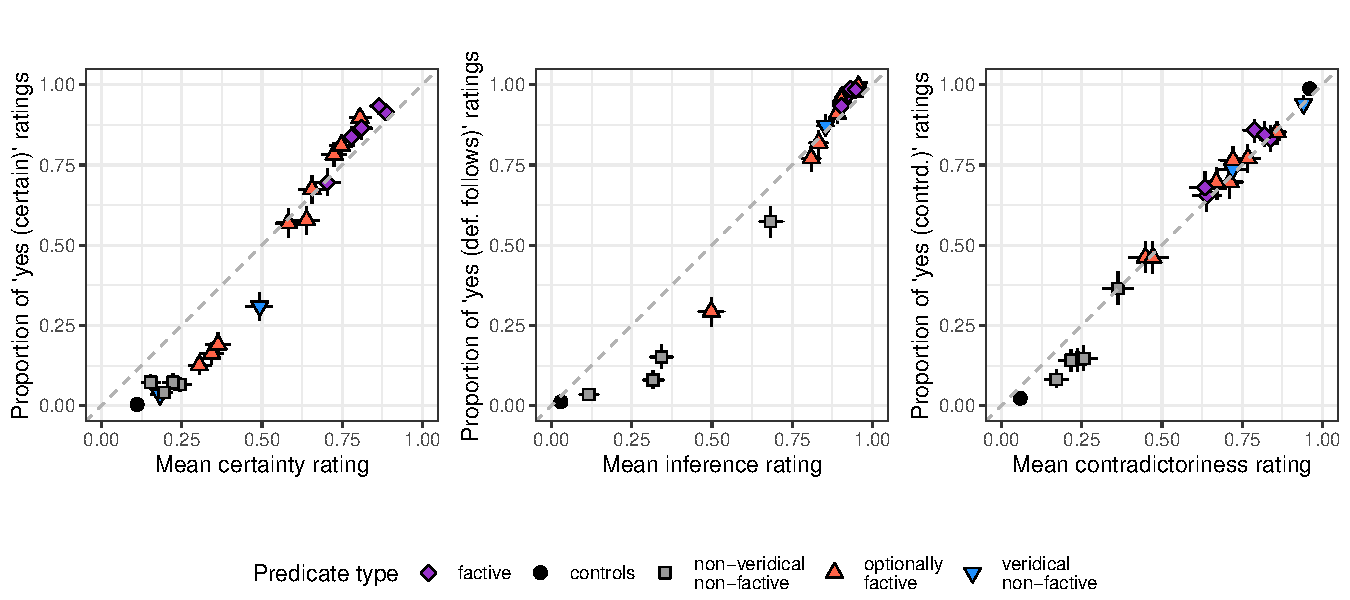
\includegraphics[width=.75\paperwidth]{../../results/compare-diagnostics-and-response-tasks/graphs/joint-comparison-plot}
   
\caption{Proportion of `yes' ratings in two-alternative forced choice task by mean ratings on gradient scale, with 95\% bootstrapped confidence intervals, collapsing over complement clauses.}
\label{f-comparison}
\end{figure}



\bibliographystyle{../cslipubs-natbib}
\bibliography{../../bibliography}

\end{document}

